\documentclass[
]{jss}

%% recommended packages
\usepackage{orcidlink,thumbpdf,lmodern}

\usepackage[utf8]{inputenc}

\author{
John Fox~\orcidlink{0000-0002-1196-8012}\\McMaster
University \And Georges Monette~\orcidlink{0000-0003-0076-5532}\\York
University
}
\title{\pkg{cv}: An \proglang{R} Package for Cross-Validating Regression
Models}

\Plainauthor{John Fox, Georges Monette}
\Plaintitle{cv: An R Package for Cross-Validating Regression Models}
\Shorttitle{\pkg{cv}: Cross-Validating Regression Models}


\Abstract{
We describe the \pkg{cv} package, which implements cross-validation for
standard \proglang{R} regression models through a uniform and simple to
use generic function. Methods for the \code{cv()} function are provided
for many commonly employed classes of statistical models, including
mixed-effects models, and it is straightforward to extend the \pkg{cv}
package by writing methods for additional classes of models. The
\code{cv()} function can also cross-validate complex model-selection
procedures, such as those that include variable transformations,
predictor selection, and selection among competing models. The
\code{cv()} function generally supports parallel computations, and the
supplied methods for linear and generalized linear models take advantage
of computational efficiencies.
}

\Keywords{cross-validation, regression analysis, model
selection, \proglang{R}}
\Plainkeywords{cross-validation, regression analysis, model
selection, R}

%% publication information
%% \Volume{50}
%% \Issue{9}
%% \Month{June}
%% \Year{2012}
%% \Submitdate{}
%% \Acceptdate{2012-06-04}

\Address{
    John Fox\\
    McMaster University\\
    Hamilton, Ontario, Canada\\
  E-mail: \email{jfox@mcmaster.ca}\\
  URL: \url{https://www.john-fox.ca/}\\~\\
      Georges Monette\\
    York University\\
    Toronto, Ontario, Canada\\
  E-mail: \email{georges@yorku.ca}\\
  URL: \url{http://blackwell.math.yorku.ca/gmonette}\\~\\
  }


% tightlist command for lists without linebreak
\providecommand{\tightlist}{%
  \setlength{\itemsep}{0pt}\setlength{\parskip}{0pt}}



\usepackage{subfig}

\usepackage{amsmath} \usepackage{amssymb}

\begin{document}



\section{Introduction}\label{introduction}

Cross-validation (CV) is an essentially simple and intuitively
reasonable approach to estimating the predictive accuracy of regression
models. CV is developed in many standard sources on regression modeling
and ``machine learning''---we particularly recommend \citet[Secs. 5.1,
5.3]{JamesEtAl:2021}---and so we will describe the method only briefly
here before taking up computational issues and some examples. See
\citet{ArlotCelisse:2010} for a wide-ranging, if technical, survey of
cross-validation and related methods that emphasizes the statistical
properties of CV.

Validating research by replication on independently collected data is a
common scientific norm. Emulating this process in a single study by
data-division is less common \citep[see, e.g.,][]{Barnard:1974}: The
data are randomly divided into two, possibly equal-size, parts; the
first part is used to develop and fit (in the language of machine
leaning, ``train'') a statistical model; and then the second part is
used to assess the adequacy of (``validate'') the model fit to the first
part of the data. Data-division, however, suffers from two problems: (1)
Dividing the data decreases the sample size and thus increases sampling
error; and (2), even more disconcertingly, the results can vary
substantially based on the random division of the data, particularly in
smaller samples. See \citet[Sec.~5.3]{Harrell:2015} for cogent remarks
about data-division and cross-validation.

Cross-validation speaks to both of these issues. In CV, the data are
randomly divided as equally as possible into several, say \(k\), parts,
called ``folds.'' The statistical model is fit \(k\) times, leaving each
fold out in turn. Each fitted model is then used to predict the response
variable for the cases in the omitted fold. A CV criterion (also termed
a ``cost'' or ``loss'' measure), such as the mean-squared error
(``MSE'') of prediction, is then computed using these predicted values.
In the extreme, \(k\) equals \(n\), the number of cases in the data,
thus omitting individual cases and refitting the model \(n\) times---a
procedure termed ``leave-one-out (LOO) cross-validation.''

Because the \(n\) models are each fit to \(n - 1\) cases, LOO CV
produces a nearly unbiased estimate of the prediction error compared
with a model fit to \(n\) cases. The \(n\) regression models are highly
statistically dependent, however, based as they are on nearly the same
data, and so the resulting estimate of prediction error has larger
variance than if the predictions from the models fit to the \(n\) data
sets were independent.

Because predictions are based on smaller data sets, each of size
approximately \(n - n/k\), estimated prediction error for \(k\)-fold CV
with \(k = 5\) or \(10\) (commonly employed choices) is more biased than
estimated prediction error for LOO CV. It is possible, however, to
correct \(k\)-fold CV for bias (see Appendix A.2).

The relative \emph{variance} of prediction error for LOO CV and
\(k\)-fold CV (with \(k < n\)) is more complicated: Because the overlap
between the data sets with each fold omitted is smaller for \(k\)-fold
CV than for LOO CV, the dependencies among the predictions are smaller
for the former than for the latter, tending to produce smaller variance
in prediction error for \(k\)-fold CV. In contrast, there are factors
that tend to inflate the variance of prediction error in \(k\)-fold CV,
including the reduced size of the data sets with each fold omitted and
the randomness induced by the selection of folds---in LOO CV the folds
are not random.

The \pkg{cv} package for \proglang{R} automates the process of
cross-validation for standard \proglang{R} statistical models. The
principal function in the package, also named \code{cv()}, has methods
for objects produced by a number of commonly employed
regression-modeling functions, including those for mixed-effects models:

\begin{CodeChunk}
\begin{CodeInput}
R> library("cv", quietly = TRUE)
R> methods("cv")
\end{CodeInput}
\begin{CodeOutput}
[1] cv.default*  cv.function* cv.glm*      cv.glmmTMB*  cv.lm*
[6] cv.lme*      cv.merMod*   cv.modList*  cv.rlm*
see '?methods' for accessing help and source code
\end{CodeOutput}
\end{CodeChunk}

The \code{cv()} function is introduced in the context of a preliminary
example in Section~\ref{preliminary-example-polynomial-regression} of
the paper.

\begin{itemize}
\item
  The \code{"lm"} and \code{"glm"} methods are for linear and
  generalized-linear models fit respectively by the standard
  \proglang{R} \code{lm()} and \code{glm()} functions.
\item
  The \code{"modList"} method for \code{cv()} cross-validates several
  competing models, not necessarily of the same class, using the same
  division of the data into folds.
\item
  Cross-validating mixed-effects models, using the \code{"glmmTMB"},
  \code{"lme"}, and \code{"merMod"} methods for \code{cv()}, involves
  special considerations that we take up in Section
  \ref{cross-validating-mixed-effects-models}.
\item
  The \code{"function"} method for \code{cv()}, discussed in Section
  \ref{cross-validating-model-specification}, cross-validates a
  potentially complex model-specification process that may, for example,
  involve choice of data transformations and predictors, or model
  selection via CV itself.
\item
  The \code{"default"} \code{cv()} method works (perhaps with a bit of
  coaxing) with many other existing regression-model classes for which
  there is an \code{update()} method that accepts a \code{data}
  argument. More generally, the \pkg{cv} package is designed to be
  extensible, as discussed in Section~\ref{extending-the-cv-package}.
\end{itemize}

A number of existing \proglang{R} packages include functions for
cross-validating regression models. In Section
\ref{comparing-cv-to-other-software-for-cross-validation}, we briefly
situate the \pkg{cv} package relative to other \proglang{R} software for
cross-validation (directly comparing \pkg{cv} to the \pkg{rsample} and
\pkg{caret} packages), and to other statistical software (in particular,
\proglang{SAS}, \proglang{Stata}, and \proglang{Python}).

An appendix to the paper describes some computational details, including
efficient CV computations for linear and generalized-linear models, and
computation of bias-corrected CV criteria.

In the interest of brevity, we won't describe all of the features of the
\pkg{cv} package here, concentrating on the aspects of the package that
are relatively novel. For example, the \code{cv()} function can perform
computations in parallel and can independently replicate a
cross-validation procedure several times. There are also data-management
facilities in the package, such as coercing the objects produced by the
\code{cv()} function into data frames for further analysis. These and
other features not discussed in this paper are taken up in the vignettes
distributed with the package, which also provide greater detail on some
topics that we do describe, such as extensions to the package.

\section{Preliminary example: Polynomial
regression}\label{preliminary-example-polynomial-regression}

The data for the example in this section are drawn from the \pkg{ISLR2}
package for \proglang{R}, associated with \citet{JamesEtAl:2021}. The
presentation here is close (though not identical) to that in the
original source \citep[ Secs. 5.1, 5.3]{JamesEtAl:2021}, and it
demonstrates the use of the \code{cv()} function.\footnote{\citet{JamesEtAl:2021}
  use the \code{cv.glm()} function in the \pkg{boot} package
  \citep{CantyRipley2022, DavisonHinkley:1997}. Despite its name,
  \code{cv.glm()} is an independent function and not a method of a
  \code{cv()} generic function. The \pkg{boot} package is part of the
  standard \proglang{R} distribution.}

The \code{Auto} data set contains information about 392 cars:

\begin{CodeChunk}
\begin{CodeInput}
R> data("Auto", package = "ISLR2")
R> summary(Auto)
\end{CodeInput}
\begin{CodeOutput}
      mpg         cylinders     displacement   horsepower        weight
 Min.   : 9.0   Min.   :3.00   Min.   : 68   Min.   : 46.0   Min.   :1613
 1st Qu.:17.0   1st Qu.:4.00   1st Qu.:105   1st Qu.: 75.0   1st Qu.:2225
 Median :22.8   Median :4.00   Median :151   Median : 93.5   Median :2804
 Mean   :23.4   Mean   :5.47   Mean   :194   Mean   :104.5   Mean   :2978
 3rd Qu.:29.0   3rd Qu.:8.00   3rd Qu.:276   3rd Qu.:126.0   3rd Qu.:3615
 Max.   :46.6   Max.   :8.00   Max.   :455   Max.   :230.0   Max.   :5140

  acceleration       year        origin                     name
 Min.   : 8.0   Min.   :70   Min.   :1.00   amc matador       :  5
 1st Qu.:13.8   1st Qu.:73   1st Qu.:1.00   ford pinto        :  5
 Median :15.5   Median :76   Median :1.00   toyota corolla    :  5
 Mean   :15.5   Mean   :76   Mean   :1.58   amc gremlin       :  4
 3rd Qu.:17.0   3rd Qu.:79   3rd Qu.:2.00   amc hornet        :  4
 Max.   :24.8   Max.   :82   Max.   :3.00   chevrolet chevette:  4
                                            (Other)           :365
\end{CodeOutput}
\end{CodeChunk}

With the exception of \code{origin} (which we don't use here), these
variables are largely self-explanatory, except possibly for units of
measurement: For details see \code{help("Auto",}
\code{package = "ISLR2")}.

\begin{CodeChunk}
\begin{figure}

{\centering \subfloat[\label{fig:mpg-horsepower-polynomials-1}]{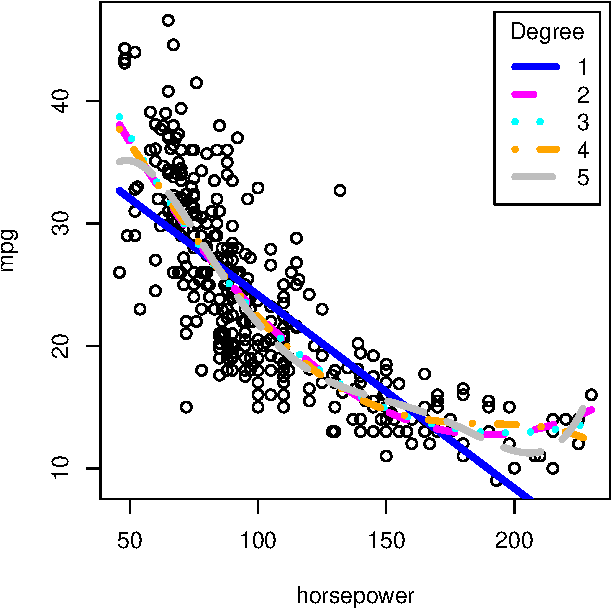
\includegraphics[width=0.45\linewidth]{Figures/mpg-horsepower-polynomials-1} }~~~\subfloat[\label{fig:mpg-horsepower-polynomials-2}]{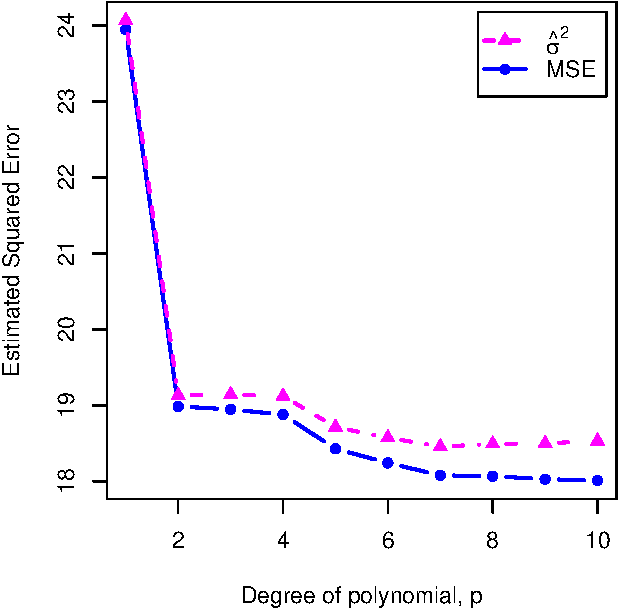
\includegraphics[width=0.45\linewidth]{Figures/mpg-horsepower-polynomials-2} }

}

\caption{(a) \code{mpg} vs. \code{horsepower} for the \code{Auto} data, showing fitted polynomials of degree 1 through 5. (b) Estimated squared error as a function of polynomial degree, $p = 1, \ldots, 10$.}\label{fig:mpg-horsepower-polynomials}
\end{figure}
\end{CodeChunk}

We'll focus on the relationship of \code{mpg} (miles per gallon) to
\code{horsepower}, as displayed in
Figure~\ref{fig:mpg-horsepower-polynomials} (a). The relationship
between the two variables is monotone, decreasing, and nonlinear.
Following \citet{JamesEtAl:2021}, we'll consider approximating the
relationship by a polynomial regression, with the degree of the
polynomial \(p\) ranging from 1 (a linear regression) to 10.\footnote{Although
  it serves to illustrate the use of CV, a polynomial is not the best
  choice here. Consider, for example, the scatterplot for
  log-transformed \code{mpg} and \code{horsepower}, produced by
  \code{plot(mpg $\sim$ horsepower, data = Auto, log = "xy")} (execution
  of which is left to the reader). We revisit the \code{Auto} data in
  Section~\ref{cross-validating-model-specification}.} Polynomial fits
for \(p = 1\) to \(5\) are shown in Figure
\ref{fig:mpg-horsepower-polynomials} (a). The linear fit is clearly
inappropriate; the fits for \(p = 2\) (quadratic) through \(4\) are very
similar; and the degree-5 polynomial may over-fit the data by chasing
one or two relatively high \code{mpg} values at the right (but see the
CV results reported below).

Figure~\ref{fig:mpg-horsepower-polynomials} (b) shows two measures of
estimated (squared) error as a function of polynomial-regression degree:
The mean-squared error (``MSE''), defined as
\(\mathsf{MSE} = \frac{1}{n}\sum_{i=1}^n (y_i - \widehat{y}_i)^2\), and
the usual residual variance, defined as
\(\widehat{\sigma}^2 = \frac{1}{n - p - 1} \sum_{i=1}^n (y_i - \widehat{y}_i)^2\).
Here \(y_i\) is the response and \(\widehat{y}_i\) the fitted value for
the \(i\)th case. The former necessarily declines with \(p\) (or, more
strictly, can't increase with \(p\)), while the latter gets slightly
larger for the largest values of \(p\), with the ``best'' value, by a
small margin, for \(p = 7\).

The generic \code{cv()} function has an \code{"lm"} method,

\begin{CodeChunk}
\begin{CodeInput}
R> args(cv:::cv.lm)
\end{CodeInput}
\begin{CodeOutput}
function (model, data = insight::get_data(model), criterion = mse,
    k = 10L, reps = 1L, seed = NULL, details = k <= 10L, confint = n >=
        400L, level = 0.95, method = c("auto", "hatvalues", "Woodbury",
        "naive"), ncores = 1L, ...)
NULL
\end{CodeOutput}
\end{CodeChunk}

which takes the following arguments:

\begin{itemize}
\item
  \code{model}, an \code{"lm"} object, the only required argument.
\item
  \code{data}, the data to which the model was fit, and which can
  usually be inferred from the \code{model} object, using the
  \code{get_data()} function from the \pkg{insight} package
  \citep{LudeckeWaggonerMakowski:2019}. The \pkg{insight} package
  provides a robust way to access model components for many classes of
  statistical models.
\item
  \code{criterion}, a function to compute the CV criterion (defaulting
  to \code{mse}).
\item
  \code{k}, the number of folds to employ (defaulting to \code{10}); the
  character value \code{"n"} or \code{"loo"} may be supplied to specify
  leave-one-out cross-validation.
\item
  \code{reps}, the number of times to repeat the CV procedure
  (defaulting to 1).
\item
  \code{seed}, the seed for \proglang{R}'s pseudo-random number
  generator; if not specified a value is randomly selected, reported,
  and saved, so that the CV procedure is replicable.
\item
  \code{confint}, whether or not to compute a confidence interval for
  the CV criterion, defaulting to \code{TRUE} if there are at least 400
  cases; a confidence interval is computed only if the CV criterion can
  be expressed as the average of casewise components (see Appendix A.2
  for details).
\item
  \code{level}, the level for the confidence interval (defaulting to
  \code{0.95}).
\item
  \code{method}, the computational method to employ: \code{"hatvalues"}
  is relevant only for LOO CV and bases computation on the hatvalues for
  the linear model; \code{"Woodbury"} employs the Woodbury matrix
  identity to compute the CV criterion with each fold deleted;
  \code{"naive"} updates the model using the \code{update()} function;
  and \code{"auto"} (the default) selects \code{"hatvalues"} for LOO CV
  and \code{"Woodbury"} for \(k\)-fold CV, both of which are much more
  efficient than directly recomputing the least-squares fit (see below
  and Appendix A.1).
\item
  \code{ncores}, the number of cores to employ for parallel computation;
  if \code{ncores = 1} (the default), the computations are not
  parallelized.
\end{itemize}

To illustrate, we perform 10-fold CV for a quadratic polynomial fit to
the \code{Auto} data:\footnote{We load the \pkg{car} package
  \citep{FoxWeisberg:2019} here for the \code{brief()} function and to
  use below.}

\begin{CodeChunk}
\begin{CodeInput}
R> library("car", quietly = TRUE)
R>
R> m.auto <- lm(mpg ~ poly(horsepower, 2), data = Auto)
R> brief(m.auto)
\end{CodeInput}
\begin{CodeOutput}
           (Intercept) poly(horsepower, 2)1 poly(horsepower, 2)2
Estimate        23.446              -120.14                44.09
Std. Error       0.221                 4.37                 4.37

 Residual SD = 4.37 on 389 df, R-squared = 0.688
\end{CodeOutput}
\begin{CodeInput}
R> (cv.auto <- cv(m.auto, confint = TRUE))
\end{CodeInput}
\begin{CodeOutput}
R RNG seed set to 623225
\end{CodeOutput}
\begin{CodeOutput}
cross-validation criterion (mse) = 19.409
\end{CodeOutput}
\begin{CodeInput}
R> summary(cv.auto)
\end{CodeInput}
\begin{CodeOutput}
10-Fold Cross Validation
method: Woodbury
criterion: mse
cross-validation criterion = 19.409
bias-adjusted cross-validation criterion = 19.386
95% CI for bias-adjusted CV criterion = (15.885, 22.887)
full-sample criterion = 18.985
\end{CodeOutput}
\end{CodeChunk}

The \texttt{print()} method for \texttt{"cv"} objects reports the CV
estimate of MSE; the \texttt{summary()} method, which we'll use
extensively in the sequel, in addition reports a bias-adjusted estimate
of the MSE (the bias adjustment is explained in Appendix A.2), and the
MSE is also computed for the original, full-sample regression. Because
the number of cases \(n = 392 < 400\) for the \code{Auto} data, we set
the argument \code{confint = TRUE} to obtain a confidence interval for
the MSE, which proves to be quite wide.

To perform LOO CV:

\begin{CodeChunk}
\begin{CodeInput}
R> summary(cv(m.auto, k = "loo"))
\end{CodeInput}
\begin{CodeOutput}
n-Fold Cross Validation
method: hatvalues
criterion: mse
cross-validation criterion = 19.248
\end{CodeOutput}
\end{CodeChunk}

The \code{"hatvalues"} method computes only the CV estimate of MSE.
Alternative methods are to use the Woodbury matrix identity or the
``naive'' approach of literally refitting the model with each case
omitted. All three methods produce exact results for a linear model
(within the precision of floating-point computations); for example:

\begin{CodeChunk}
\begin{CodeInput}
R> summary(cv(m.auto, k = "loo", method = "naive", confint = TRUE))
\end{CodeInput}
\begin{CodeOutput}
n-Fold Cross Validation
method: naive
criterion: mse
cross-validation criterion = 19.248
bias-adjusted cross-validation criterion = 19.248
95% CI for bias-adjusted CV criterion = (15.779, 22.717)
full-sample criterion = 18.985
\end{CodeOutput}
\end{CodeChunk}

The \code{"naive"} and \code{"Woodbury"} methods also return the
bias-adjusted estimate of MSE (and a confidence interval around it)
along with the full-sample MSE, but bias isn't an issue for LOO CV.

This is a small regression problem and all three computational
approaches are essentially instantaneous, but it is still of interest to
investigate their relative speed. In the following comparison, we
include the \code{cv.glm()} function from the \pkg{boot} package, which
takes the naive approach, and for which we have to fit the linear model
as an equivalent Gaussian GLM; the output shown is for the CV estimate
of MSE and the bias-corrected CV estimate. We use the
\code{microbenchmark()} function from the package of the same name
\citep{Mersmann:2023} for the timings:

\begin{CodeChunk}
\begin{CodeInput}
R> m.auto.glm <- glm(mpg ~ poly(horsepower, 2), data = Auto)
R> boot::cv.glm(Auto, m.auto.glm)$delta
\end{CodeInput}
\begin{CodeOutput}
[1] 19.248 19.248
\end{CodeOutput}
\begin{CodeInput}
R> set.seed(19412)
R> print(microbenchmark::microbenchmark(
+   hatvalues = cv(m.auto, k = "loo"),
+   Woodbury = cv(m.auto, k = "loo", method = "Woodbury"),
+   naive = cv(m.auto, k = "loo", method = "naive"),
+   cv.glm = boot::cv.glm(Auto, m.auto.glm),
+   times = 10, unit = "relative"), signif = 3)
\end{CodeInput}
\begin{CodeOutput}
Warning in microbenchmark::microbenchmark(hatvalues = cv(m.auto, k = "loo"), :
less accurate nanosecond times to avoid potential integer overflows
\end{CodeOutput}
\begin{CodeOutput}
Unit: relative
      expr    min     lq   mean median     uq   max neval cld
 hatvalues   1.00   1.00   1.00   1.00   1.00  1.00    10 a
  Woodbury   7.47   7.15   5.77   6.74   6.62  2.35    10 a
     naive 124.00 119.00  98.20 112.00 111.00 47.50    10  b
    cv.glm 217.00 207.00 172.00 197.00 198.00 75.20    10   c
\end{CodeOutput}
\end{CodeChunk}

On our computer, using the hatvalues is about an order of magnitude
faster than employing Woodbury matrix updates, and more than two orders
of magnitude faster than refitting the model.\footnote{Out of
  impatience, we asked \code{microbenchmark()} to execute each command
  only 10 times rather than the default 100. With the exception of the
  last column, the output is self-explanatory. The last column shows
  which methods have average timings that are statistically
  distinguishable (as indicated by different letters). Because of the
  small number of repetitions (i.e., 10), the \code{"hatvalues"} and
  \code{"Woodbury"} methods aren't distinguishable, but the difference
  between these methods persists when we perform more repetitions---we
  invite the patient reader to redo this computation with the default
  \code{times = 100} repetitions.}

\subsection{Comparing competing
models}\label{comparing-competing-models}

The \code{cv()} function also has a method that can be applied to a list
of regression models for the same data, composed using the
\code{models()} function. For \(k\)-fold CV, the same folds are used for
the competing models, which reduces random error in their comparison.
This result can also be obtained by specifying a common seed for
\proglang{R}'s random-number generator while applying \code{cv()}
separately to each model, but employing a list of models is more
convenient for both \(k\)-fold and LOO CV (where there is no random
component to the composition of the \(n\) folds).

We illustrate with the polynomial regression models of varying degree
for the \code{Auto} data, beginning by fitting and saving the 10 models:

\begin{CodeChunk}
\begin{CodeInput}
R> mlist <- vector(10, mode = "list")
R> for (p in 1:10) mlist[[p]] <- lm(mpg ~ poly(horsepower, p), data = Auto)
R> names(mlist) <- paste0("m.", 1:10)
R> mlist[2]
\end{CodeInput}
\begin{CodeOutput}
$m.2

Call:
lm(formula = mpg ~ poly(horsepower, p), data = Auto)

Coefficients:
         (Intercept)  poly(horsepower, p)1  poly(horsepower, p)2
                23.4                -120.1                  44.1
\end{CodeOutput}
\end{CodeChunk}

where, for example, \code{mlist[2]} is the quadratic fit.

We then apply \code{cv()} to the list of 10 models for both 10-fold and
LOO CV (the \code{data} argument to \code{cv()} is required):

\begin{CodeChunk}
\begin{CodeInput}
R> mlist <- models(mlist)
R>
R> cv.auto.10 <- cv(mlist, data = Auto, seed = 2120)
R> cv.auto.10[2]
\end{CodeInput}
\begin{CodeOutput}
Model m.2:
cross-validation criterion = 19.346
\end{CodeOutput}
\begin{CodeInput}
R> cv.auto.loo <- cv(mlist, data = Auto, k = "loo")
R> cv.auto.loo[2]
\end{CodeInput}
\begin{CodeOutput}
Model m.2:
cross-validation criterion = 19.248
\end{CodeOutput}
\end{CodeChunk}

The \code{models()} function takes an arbitrary number of regression
models as its arguments, which are optionally named, to create a
\code{"modList"} object. Alternatively, as here, we can supply a
pre-constructed, optionally named, list of models as the single argument
to \code{models()}. To visualize the results, comparing the models, we
invoke the \code{plot()} method for the \code{"cvModList"} objects
returned by \code{cv()} (see Figure
\ref{fig:polynomial-regression-CV-graph-2}):\footnote{The objects
  \code{cv.auto.10} and \code{cv.auto.loo} do not include confidence
  intervals for the CV MSE estimates because, as we explained, there are
  fewer than 400 cases in the \code{Auto} data. Consequently, confidence
  intervals are not shown in the graphs in Figure
  \ref{fig:polynomial-regression-CV-graph-2}. We can force \texttt{cv()}
  to compute confidence intervals by adding the argument
  \texttt{confint\ =\ TRUE}; we invite the reader to do this and to
  verify that the resulting confidence intervals are very broad, as was
  the case for the quadratic model fit to the \code{Auto} data in the
  preceding section.}

\begin{CodeChunk}
\begin{CodeInput}
R> plot(cv.auto.10, main = "Polynomial Regressions, 10-Fold CV",
+      axis.args = list(labels = 1:10), xlab = "Degree of Polynomial, p")
R> plot(cv.auto.loo, main = "Polynomial Regressions, LOO CV",
+      axis.args = list(labels = 1:10), xlab = "Degree of Polynomial, p")
\end{CodeInput}
\begin{figure}

{\centering \subfloat[\label{fig:polynomial-regression-CV-graph-2-1}]{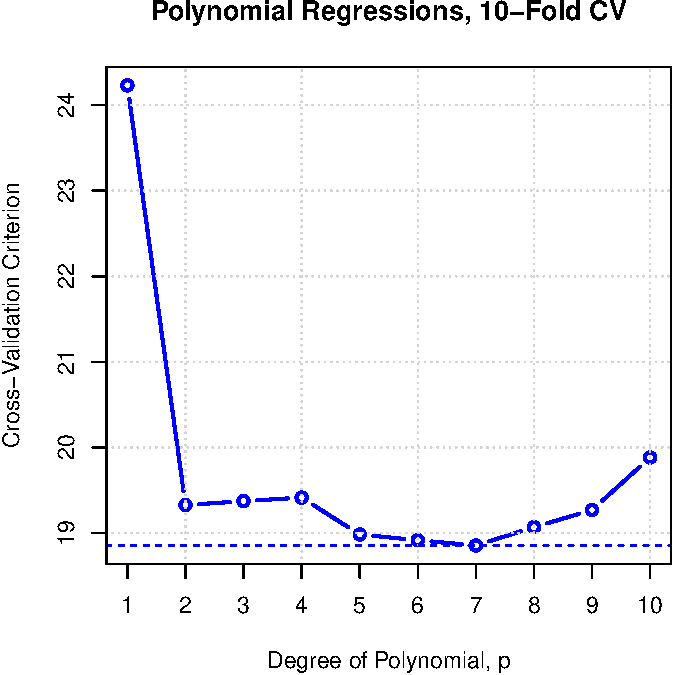
\includegraphics[width=0.5\linewidth]{Figures/polynomial-regression-CV-graph-2-1} }~~~\subfloat[\label{fig:polynomial-regression-CV-graph-2-2}]{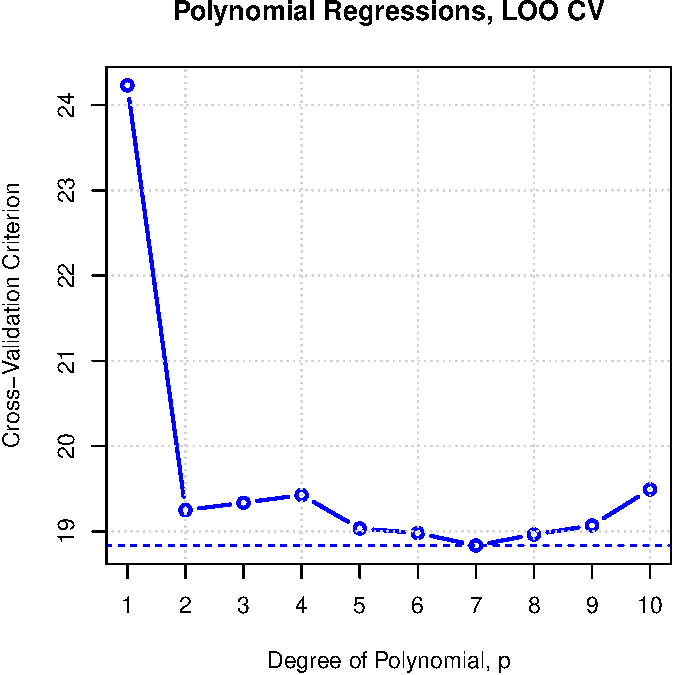
\includegraphics[width=0.5\linewidth]{Figures/polynomial-regression-CV-graph-2-2} }

}

\caption[Cross-validated (a) 10-fold and (b) LOO MSE as a function of polynomial degree, $p = 1, 2, \ldots, 10$]{Cross-validated (a) 10-fold and (b) LOO MSE as a function of polynomial degree, $p = 1, 2, \ldots, 10$.}\label{fig:polynomial-regression-CV-graph-2}
\end{figure}
\end{CodeChunk}

In this example, 10-fold and LOO CV produce generally similar results,
and also results that are similar to those produced by the estimated
error variance \(\widehat{\sigma}^2\) for each model (cf., Figure
\ref{fig:mpg-horsepower-polynomials} (b) on page
\pageref{fig:mpg-horsepower-polynomials}), except for the highest-degree
polynomials, where the CV results more clearly suggest over-fitting.
\newpage

\section{Cross-validating mixed-effects
models}\label{cross-validating-mixed-effects-models}

The fundamental analogy for cross-validation is to the collection of new
data. That is, predicting the response in each fold from the model fit
to data in the other folds is like using the model fit to all of the
data to predict the response for new cases from the values of the
predictors for those new cases. As we explained, the application of this
idea to independently sampled cases is straightforward.

In contrast, mixed-effects models are fit to \emph{dependent} data, in
which cases are clustered, such as hierarchical data, where the clusters
comprise higher-level units (e.g., students clustered in schools), or
longitudinal data, where the clusters are individuals and the cases are
repeated observations on the individuals over time.\footnote{There are,
  however, more complex situations that give rise to so-called
  \emph{crossed} (rather than \emph{nested}) random effects. For
  example, consider students within classes within schools. In primary
  schools, students typically are in a single class, and so classes are
  nested within schools. In secondary schools, however, students
  typically take several classes and students who are together in a
  particular class may not be together in other classes; consequently,
  random effects based on classes within schools are crossed. The
  \code{lmer()} function in the \pkg{lme4} package, for example, is
  capable of modeling both nested and crossed random effects, and the
  \code{cv()} methods for mixed models in the \pkg{cv} package pertain
  to both nested and crossed random effects. We present an example of
  crossed random effects in the \pkg{cv} package vignette on mixed
  models.}

We can think of two approaches to applying cross-validation to clustered
data:\footnote{We subsequently discovered that \citet[Section
  8]{Vehtari:2023} makes similar points.}

\begin{enumerate}
\def\labelenumi{\arabic{enumi}.}
\item
  Treat CV as analogous to predicting the response for one or more cases
  in a \emph{newly observed cluster}. In this instance, the folds
  comprise one or more whole clusters; we refit the model with all of
  the cases in clusters in the current fold removed; and then we predict
  the response for the cases in clusters in the current fold. These
  predictions are based only on fixed effects because the random effects
  for the omitted clusters are construed to be unknown, as they would be
  for data on cases in newly observed clusters.
\item
  Treat CV as analogous to predicting the response for a newly observed
  case in an \emph{existing cluster}. In this instance, the folds
  comprise one or more individual cases, and the predictions can use
  both the fixed and random effects---so-called ``best-linear-unbiased
  predictors'' or ``BLUPs.''
\end{enumerate}

\subsection{Example: The High-School and Beyond
data}\label{example-the-high-school-and-beyond-data}

Following their use by \citet{RaudenbushBryk:2002}, data from the 1982
\emph{High School and Beyond} (``HSB'') survey have become a staple of
the literature on mixed-effects models. The HSB data are used by
\citet[Sec.~7.2.2]{FoxWeisberg:2019} to illustrate the application of
linear mixed models to hierarchical data, and we'll closely follow their
example here.

The HSB data are included in the \code{MathAchieve} and
\code{MathAchSchool} data sets in the \pkg{nlme} package
\citep{PinheiroBates:2000}. \code{MathAchieve} comprises
individual-level data on 7185 students in 160 high schools, and
\code{MathAchSchool} contains school-level data:

\begin{CodeChunk}
\begin{CodeInput}
R> data("MathAchieve", package = "nlme")
R> dim(MathAchieve)
\end{CodeInput}
\begin{CodeOutput}
[1] 7185    6
\end{CodeOutput}
\begin{CodeInput}
R> head(MathAchieve, 3)
\end{CodeInput}
\begin{CodeOutput}
Grouped Data: MathAch ~ SES | School
  School Minority    Sex    SES MathAch MEANSES
1   1224       No Female -1.528   5.876  -0.428
2   1224       No Female -0.588  19.708  -0.428
3   1224       No   Male -0.528  20.349  -0.428
\end{CodeOutput}
\begin{CodeInput}
R> tail(MathAchieve, 3)
\end{CodeInput}
\begin{CodeOutput}
Grouped Data: MathAch ~ SES | School
     School Minority    Sex    SES MathAch MEANSES
7183   9586       No Female  1.332  19.641   0.627
7184   9586       No Female -0.008  16.241   0.627
7185   9586       No Female  0.792  22.733   0.627
\end{CodeOutput}
\begin{CodeInput}
R> data("MathAchSchool", package = "nlme")
R> dim(MathAchSchool)
\end{CodeInput}
\begin{CodeOutput}
[1] 160   7
\end{CodeOutput}
\begin{CodeInput}
R> head(MathAchSchool, 2)
\end{CodeInput}
\begin{CodeOutput}
     School Size Sector PRACAD DISCLIM HIMINTY MEANSES
1224   1224  842 Public   0.35   1.597       0  -0.428
1288   1288 1855 Public   0.27   0.174       0   0.128
\end{CodeOutput}
\begin{CodeInput}
R> tail(MathAchSchool, 2)
\end{CodeInput}
\begin{CodeOutput}
     School Size   Sector PRACAD DISCLIM HIMINTY MEANSES
9550   9550 1532   Public   0.45   0.791       0   0.059
9586   9586  262 Catholic   1.00  -2.416       0   0.627
\end{CodeOutput}
\end{CodeChunk}

The first few students are in school number 1224 and the last few in
school 9586.

We'll use only the \code{School}, \code{SES} (students' socioeconomic
status), and \code{MathAch} (their score on a standardized
math-achievement test) variables in the \code{MathAchieve} data set, and
\code{Sector} (\code{"Catholic"} or \code{"Public"}) in the
\code{MathAchSchool} data set.

Some data-management is required before fitting a mixed-effects model to
the HSB data:

\begin{CodeChunk}
\begin{CodeInput}
R> HSB <- MathAchieve
R> HSB <- merge(MathAchSchool[, c("School", "Sector")],
+              HSB[, c("School", "SES", "MathAch")], by = "School")
R> names(HSB) <- tolower(names(HSB))
R> HSB <- within(HSB, {
+   mean.ses <- ave(ses, school)
+   cses <- ses - mean.ses
+ })
\end{CodeInput}
\end{CodeChunk}

In the process, we merge variables from the school-level and
student-level data sets, and create two new school-level variables:
\code{mean.ses}, which is the average SES for students in each school;
and \code{cses}, which is the individual students' SES centered at their
school means. For details, see \citet[Sec.~7.2.2]{FoxWeisberg:2019}.

Still following Fox and Weisberg, we proceed to use the \code{lmer()}
function in the \pkg{lme4} package \citep{BatesEtAl:2015} to fit a mixed
model for math achievement to the HSB data (summarizing the model with
the \code{S()} function from the \pkg{car} package):

\begin{CodeChunk}
\begin{CodeInput}
R> library("lme4", quietly = TRUE)
R> hsb.lmer <- lmer(mathach ~ mean.ses*cses + sector*cses
+                    + (cses | school), data = HSB)
R> S(hsb.lmer, brief = TRUE)
\end{CodeInput}
\begin{CodeOutput}

Estimates of Fixed Effects:
                    Estimate Std. Error z value Pr(>|z|)
(Intercept)           12.128      0.199   60.86  < 2e-16
mean.ses               5.333      0.369   14.45  < 2e-16
cses                   2.945      0.156   18.93  < 2e-16
sectorCatholic         1.227      0.306    4.00  6.2e-05
mean.ses:cses          1.039      0.299    3.48  0.00051
cses:sectorCatholic   -1.643      0.240   -6.85  7.3e-12

Estimates of Random Effects (Covariance Components):
 Groups   Name        Std.Dev. Corr
 school   (Intercept) 1.543
          cses        0.318    0.39
 Residual             6.060

Number of obs: 7185, groups:  school, 160

logLik     df    AIC    BIC
-23252     10  46524  46592
\end{CodeOutput}
\end{CodeChunk}

We can then cross-validate at the cluster (i.e., school) level,

\begin{CodeChunk}
\begin{CodeInput}
R> summary(cv(hsb.lmer, k = 10, clusterVariables = "school", seed = 5240))
\end{CodeInput}
\begin{CodeOutput}
R RNG seed set to 5240
\end{CodeOutput}
\begin{CodeOutput}
10-Fold Cross Validation based on 160 {school} clusters
criterion: mse
cross-validation criterion = 39.157
bias-adjusted cross-validation criterion = 39.148
95% CI for bias-adjusted CV criterion = (38.066, 40.231)
full-sample criterion = 39.006
\end{CodeOutput}
\end{CodeChunk}

or at the case (i.e., student) level,

\begin{CodeChunk}
\begin{CodeInput}
R> summary(cv(hsb.lmer, seed = 1575))
\end{CodeInput}
\begin{CodeOutput}
R RNG seed set to 1575
\end{CodeOutput}
\begin{CodeOutput}
Warning in checkConv(attr(opt, "derivs"), opt$par, ctrl = control$checkConv, :
Model failed to converge with max|grad| = 0.00587207 (tol = 0.002, component 1)
\end{CodeOutput}
\begin{CodeOutput}
boundary (singular) fit: see help('isSingular')
\end{CodeOutput}
\begin{CodeOutput}
10-Fold Cross Validation
criterion: mse
cross-validation criterion = 37.445
bias-adjusted cross-validation criterion = 37.338
95% CI for bias-adjusted CV criterion = (36.288, 38.388)
full-sample criterion = 36.068
\end{CodeOutput}
\end{CodeChunk}

For cluster-level CV, the \code{clusterVariables} argument tells
\code{cv()} how the clusters are defined. Were there more than one
clustering variable, say classes within schools, these would be provided
as a character vector of variable names:
\code{clusterVariables = c("school", "class")}. For cluster-level CV,
the default is \code{k = "loo"}, that is, leave one cluster out at a
time; we instead specify \code{k = 10} folds of clusters, each fold
therefore comprising \(160/10 = 16\) schools.

If the \code{clusterVariables} argument is omitted, then case-level CV
is employed, with \code{k = 10} folds as the default, here each with
\(7185/10 \approx 719\) students. Notice that one of the 10 models refit
with a fold removed failed to converge. Convergence problems are common
in mixed-effects modeling. The issue here is that an estimated variance
component is close to or equal to 0, which is at a boundary of the
parameter space. That shouldn't disqualify the fitted model for the kind
of prediction required for cross-validation.

\code{cv()} also has methods for mixed models fit by the \code{glmer()}
function in the \pkg{lme4} package, the \code{lme()} function in the
\pkg{nlme} package \citep{PinheiroBates:2000}, and the \code{glmmTMB()}
function in the \pkg{glmmTMB} package \citep{BrooksEtAl}, along with a
simple procedure for extending \code{cv()} to other classes of
mixed-effects models. See the vignettes in the \pkg{cv} package for
details.

\subsection{Example: Contrasting cluster-based and case-based
CV}\label{example-contrasting-cluster-based-and-case-based-cv}

In this section, we introduce four artificial data sets that exemplify
aspects of cross-validation particular to hierarchical models. Using
these data sets, we show that model comparisons employing cluster-based
and those employing case-based cross-validation may not agree on a
``best'' model. Furthermore, commonly used measures of fit, such as
mean-squared error, do not necessarily become smaller as models become
larger, even when the models are nested, and even when the measure of
fit is computed for the whole data set.

The four data sets differ in the magnitude of between-cluster variation
compared to within-cluster variation. They serve to illustrate how
fitting mixed models, and, consequently, the cross-validation of mixed
models, is sensitive to relative variation, which affects the degree of
shrinkage of within-cluster estimates of effects towards between-cluster
estimates.

The purpose of this section is to explain some of the complexities of
cross-validating mixed-effects models, which motivates the approach that
we take for mixed models in the \pkg{cv} package. The examples in this
section introduce no features of the \pkg{cv} package that we haven't
already encountered, and the generation of data for these examples
involves unenlightening data management. Consequently, we don't show the
code for data generation, model fitting, and graphs in this
section.\footnote{The code for this section is in the complementary
  materials for the paper. We used the \code{glmmTMB()} function in the
  \pkg{glmmTMB} package \citep{BrooksEtAl} for the models fit here
  because, in our experience, it is more likely to converge than
  functions in the \pkg{nlme} and the \pkg{lme4} packages for models
  with low between-cluster variation. We used the \pkg{lattice}
  \citep{Sarkar:2008} and \pkg{latticeExtra} \citep{SarkarAndrews:2022}
  packages for the graphs.}

Consider a researcher studying the effect of the dosage \(x\) of a drug
on the severity of symptoms \(y\) for a hypothetical disease. The
researcher has longitudinal data on 20 patients, each of whom was
observed on 5 occasions in which patients received different dosages of
the drug. The data are observational, with dosages prescribed by the
patients' physicians, so that patients who were more severely affected
by the disease received higher dosages of the drug.

Within patients, higher dosages are generally associated with a
reduction in symptoms. Between patients, however, higher dosages are
associated with higher levels of symptoms. A plausible mechanism is a
reversal of causality: Within patients, higher dosages alleviate
symptoms, but, between patients, higher morbidity causes the
prescription of higher dosages.

To generate the four data sets, we first constructed a template data set
from a population with a between-patient effect of dosage of \(1.0\) and
a within-patient effect of \(-0.5\). We then applied four different
multipliers to the between-patient standard deviation from the
regression line of patient centroids. The resulting data sets, shown in
Figure~\ref{fig:plot1}, differ in the between-patient variation of
patient centroids from a common between-patient regression line,
exhibiting a progression from low to high variation around the common
regression line. Each patient has the same relative configuration of
dosages and symptoms in each of the four data sets. To help visualize
the structure of the data, estimated 50\% Gaussian concentration
ellipses are shown for each patient.

\begin{CodeChunk}
\begin{figure}

{\centering 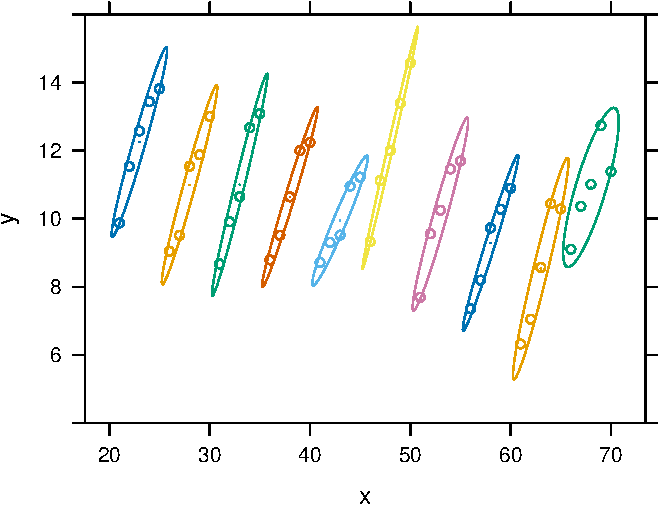
\includegraphics[width=0.75\linewidth]{Figures/plot1-1}

}

\caption[Data sets showing identical within-patient configurations with increasing between-patient variation]{Data sets showing identical within-patient configurations with increasing between-patient variation. The labels above each panel show the ratio of between-patient SD to within-patient SD. The ellipses are estimated 50\% Gaussian concentration ellipses for each patient. The population between-patient regression line, $\E(y) = 10 + x$, is shown in each panel, where $y$ is symptoms and $x$ is dosage.}\label{fig:plot1}
\end{figure}
\end{CodeChunk}

Using data like these, a researcher may attempt to obtain an estimate of
the within-patient effect of dosage by fitting mixed models with a
random intercept. We will illustrate how this approach results in
estimates that are highly sensitive to the relative variation at the two
levels of the mixed model by considering four models, all of which
include a random intercept. The first three models are sequentially
nested in their fixed effects: (1) \code{~ 1}, intercept only; (2)
\code{~ 1 + x}, intercept and effect of \code{x}; and (3)
\code{~ 1 + x + xm}, intercept, effect of \code{x}, and a contextual
variable, \code{xm}, consisting of the within-patient mean of \code{x}.
The final model, (4) \code{~ 1 + I(x - xm)}, uses an intercept and the
centered-within-group variable \code{x - xm}. We thus fit four models to
each of the four data sets for a total of 16 models.

We proceed to obtain predictions from each model (1) using only the
fixed effects, as for cross-validation based on clusters (i.e.,
patients), and (2) using both fixed and random effects---that is, the
BLUPs---as for cross-validation based on cases (i.e., occasions within
patients). The fixed- and random-effects predictions from these models
are displayed in Figure~\ref{fig:plot-fits-combined} along with a
summary of the data using 50\% concentration ellipses (see the top row
of the figure).

\begin{CodeChunk}
\begin{figure}

{\centering 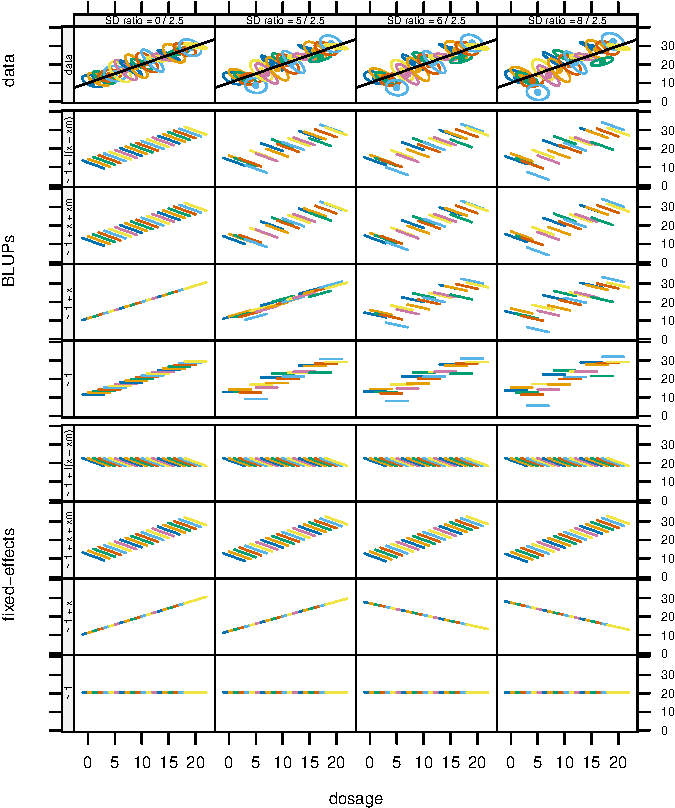
\includegraphics[width=1\linewidth]{Figures/plot-fits-combined-1}

}

\caption[Fixed- and random-effect predictions (BLUPs) using each model applied to data sets with varying between- and within-patient standard-deviation ratios]{Fixed- and random-effect predictions (BLUPs) using each model applied to data sets with varying between- and within-patient standard-deviation ratios. The top row shows summaries of the within-patient data using estimated 50\% concentration ellipses, along with the patient centroids.}\label{fig:plot-fits-combined}
\end{figure}
\end{CodeChunk}

Data sets with relatively low between-patient variation result in strong
shrinkage of fixed-effects predictions, and also of BLUPs, towards the
between-patient relationship between \code{y} and \code{x} in the model
with an intercept and \code{x} as fixed-effect predictors,
\code{~ 1 + x}. The inclusion of the contextual variable \code{xm} in
the model corrects this problem.

Although the BLUPs fit the observed data more closely than predictions
based on fixed effects alone, the slopes of within-patient BLUPs do not
conform to the within-patient slopes for the \code{~ 1 + x} model in the
two data sets with the smallest between-patient variation. For data with
a small between-patient variation, fixed-effects predictions for the
\code{~ 1 + x} model have a slope that is close to the between-patient
slope but provide better overall predictions than the fixed-effect
predictions for data sets with larger between-subject variation. With
data whose between-patient variation is relatively large, predictions
based on the model with a common intercept and slope for all clusters
are very poor---indeed, much worse than the fixed-effects-only
predictions based on the simpler random-intercept model.

We therefore anticipate (and show later in this section) that case-based
cross-validation may prefer the intercept-only model, \code{~ 1} to the
larger \code{~ 1 + x} model when the between-cluster variation is
relatively small, but that cluster-based cross-validation will prefer
the latter to the former. We will discover that case-based
cross-validation prefers the \code{~ 1 + x} model to the \code{~ 1}
model for the ``5 / 2.5'' data set, but cluster-based cross-validation
prefers the latter model to the former. The situation is entirely
reversed with the ``8 / 2.5'' data set.

The third model, \code{~ 1 + x + xm}, includes a contextual effect of
\code{x}---that is, the cluster mean \code{xm}---along with \code{x},
the intercept in the fixed-effect part of the model, and a random
intercept. This model is equivalent to fitting
\code{y ~ I(x - xm) + xm + (1 | patient)}, which is the model that
generated the data. The fit of the mixed model \code{~ 1 + x + xm} is
consequently similar to that of a fixed-effects-only model with \code{x}
and a categorical predictor for individual patients (i.e.,
\code{y ~ factor(patient) + x}, treating patients as a factor, and not
shown here).

We next carry out case-based cross-validation, which, as we have
explained, is based on both fixed and predicted random effects (i.e.,
BLUPs), and cluster-based cross-validation, which is based on fixed
effects only.\footnote{In order to reduce between-model random
  variability in comparisons of models on the same data set, we applied
  \code{cv()} to a list of models created by the \code{models()}
  function (introduced previously), performing cross-validation with the
  same folds for each model.} The results for all data sets, using both
cluster-based and case-based cross-validation, are assembled in Figure
\ref{fig:cross-validation-data-plot}.

\begin{CodeChunk}
\begin{figure}

{\centering 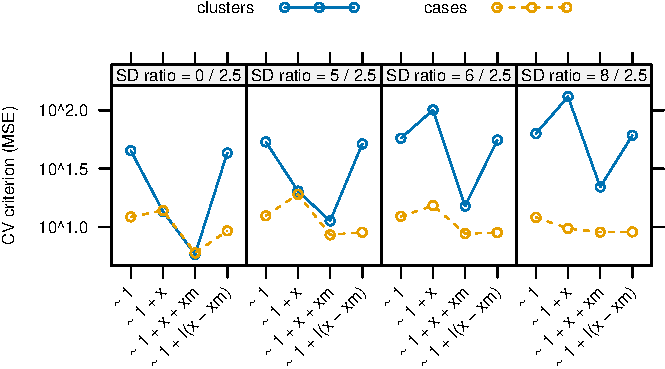
\includegraphics[width=0.75\linewidth]{Figures/cross-validation-data-plot-1}

}

\caption[10-fold cluster- and case-based cross-validation comparing mixed models with random intercepts and various fixed effects]{10-fold cluster- and case-based cross-validation comparing mixed models with random intercepts and various fixed effects.}\label{fig:cross-validation-data-plot}
\end{figure}
\end{CodeChunk}

In summary, when between-cluster variation is relatively large, the
model \code{~ 1 + x}, with \code{x} alone and without the contextual
mean \code{xm} of \code{x}, is assessed as fitting very poorly by
cluster-based CV, but relatively much better by case-based CV. In all of
our examples, the model \code{~ 1 + x + xm}, which includes both
\code{x} and its contextual mean, produces better results using both
cluster-based and case-based CV. These conclusions are consistent with
our observations based on graphing predictions from the various models
(in Figure~\ref{fig:plot-fits-combined} on page
\pageref{fig:plot-fits-combined}), and they illustrate the desirability
of assessing mixed-effect models at different hierarchical levels.

\section{Cross-validating model
specification}\label{cross-validating-model-specification}

As \citet[Sec.~7.10.2: ``The Wrong and Right Way to Do
Cross-validation'']{HastieTibshiraniFriedman:2009} explain, if the whole
data are used to specify or fine-tune a statistical model, then
subsequent cross-validation of the model is intrinsically misleading,
because the model is selected to fit the whole data, including the part
of the data that remains when each fold is removed. Statistical modeling
is partly a craft, and one could imagine applying that craft
independently to successive partial data sets, each with a fold removed.
The resulting procedure would be tedious, though possibly worth the
effort, but it would also be difficult to realize in practice: After
all, we can hardly erase our memory of statistical modeling choices
between analyzing partial data sets. Alternatively, if we're able to
automate the process of model specification, then we can more
realistically apply CV mechanically.

The \code{"function"} method for \code{cv()} cross-validates a
model-specification process in a general manner. Functions for four such
model-specification processes are included in the package:
\code{selectStepAIC()}, based on the \code{stepAIC()} function in the
\pkg{MASS} package \citep{VenablesRipley:2002}, performs stepwise
predictor selection for regression models; \code{selectTrans()}, based
on the \code{powerTransform()} function in the \pkg{car} package,
transforms predictors and the response in a regression model towards
normality; \code{selectTransStepAIC()}---the use of which we illustrate
in the current section---performs both of these procedures sequentially;
and \code{selectModelList()}---also illustrated in the current
section---uses CV both to select one of several competing models, and
then, recursively, to estimate prediction error for the selected model,
a process that we term ``meta cross-validation.''\footnote{In a vignette
  on extending the \pkg{cv} package, we explain how to specify
  additional model-selection procedures.}

\subsection[Example: Data transformation and predictor selection for the Auto
data]{Example: Data transformation and predictor selection for the
\code{Auto}
data}\label{example-data-transformation-and-predictor-selection-for-the-auto-data}

To illustrate cross-validation of model specification, we return to the
\code{Auto} data set:\footnote{This example benefits from an email
  conversation with Bill Venables, who of course isn't responsible for
  the use to which we've put his insightful remarks.}

\begin{CodeChunk}
\begin{CodeInput}
R> names(Auto)
\end{CodeInput}
\begin{CodeOutput}
[1] "mpg"          "cylinders"    "displacement" "horsepower"   "weight"
[6] "acceleration" "year"         "origin"       "name"
\end{CodeOutput}
\begin{CodeInput}
R> xtabs(~ year, data = Auto)
\end{CodeInput}
\begin{CodeOutput}
year
70 71 72 73 74 75 76 77 78 79 80 81 82
29 27 28 40 26 30 34 28 36 29 27 28 30
\end{CodeOutput}
\begin{CodeInput}
R> xtabs(~ origin, data = Auto)
\end{CodeInput}
\begin{CodeOutput}
origin
  1   2   3
245  68  79
\end{CodeOutput}
\begin{CodeInput}
R> xtabs(~ cylinders, data = Auto)
\end{CodeInput}
\begin{CodeOutput}
cylinders
  3   4   5   6   8
  4 199   3  83 103
\end{CodeOutput}
\end{CodeChunk}

The \code{Auto} data appeared in a preliminary example in Section
\ref{preliminary-example-polynomial-regression}, where we employed CV to
inform the selection of the degree of a polynomial regression of
\code{mpg} on \code{horsepower}. Here, we consider more generally the
problem of predicting \code{mpg} from the other variables in the
\code{Auto} data. We begin with a bit of data management, and then
examine the pairwise relationships among the numeric variables in the
data set (Figure~\ref{fig:Auto-explore-scatterplot-matrix}, produced by
the \code{scatterplotMatrix()} function in the \pkg{car} package); in
each panel, the solid line shows the linear least-squares fit and the
broken line is for a nonparametric regression:

\begin{CodeChunk}
\begin{CodeInput}
R> Auto$cylinders <- factor(Auto$cylinders,
+                          labels = c("3-4", "3-4", "5-6", "5-6", "8"))
R> Auto$year <- as.factor(Auto$year)
R> Auto$origin <- factor(Auto$origin,
+                       labels = c("America", "Europe", "Japan"))
R> rownames(Auto) <- make.names(Auto$name, unique = TRUE)
R> Auto$name <- NULL
R>
R> scatterplotMatrix(~ mpg + displacement + horsepower + weight
+                   + acceleration,
+                   smooth = list(spread = FALSE), data = Auto, pch= ".")
\end{CodeInput}
\begin{figure}

{\centering 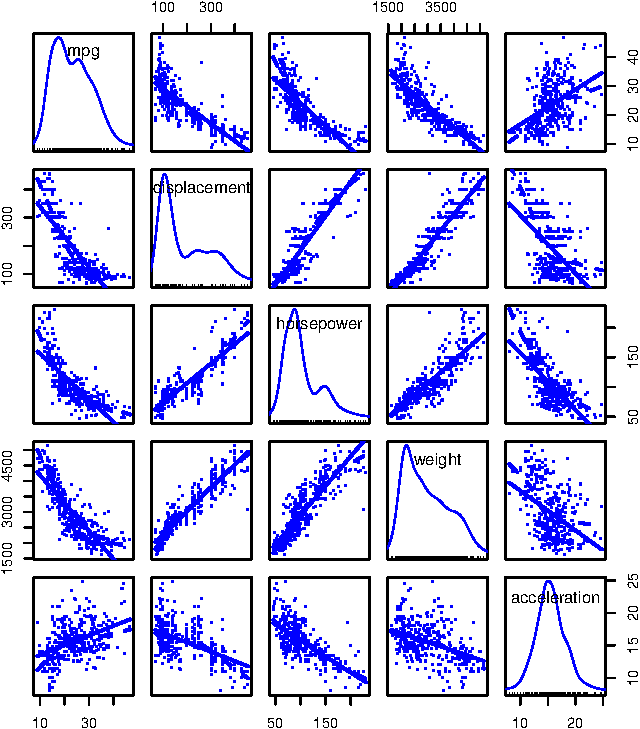
\includegraphics[width=0.95\linewidth]{Figures/Auto-explore-scatterplot-matrix-1}

}

\caption[Scatterplot matrix for the numeric variables in the \code{Auto} data]{Scatterplot matrix for the numeric variables in the \code{Auto} data.}\label{fig:Auto-explore-scatterplot-matrix}
\end{figure}
\end{CodeChunk}

A comment before we proceed: \code{origin} is clearly categorical and so
converting it to a factor is natural, but we could imagine treating
\code{cylinders} and \code{year} as numeric predictors. There are,
however, only 5 distinct values of \code{cylinders}, ranging from 3 to
8, but cars with 3 or 5 cylinders are rare, and none of the cars has 7
cylinders. There are similarly only 13 distinct years between 1970 and
1982 in the data, and the relationship between \code{mpg} and
\code{year} is difficult to characterize.\footnote{Making the decision
  to treat \code{year} as a factor on this basis could be construed as
  cheating in the current context, which illustrates the difficulty of
  automating the whole model-selection process. It's rarely desirable,
  in our opinion, to forgo exploration of the data to ensure the purity
  of model validation. We believe, however, that it's still useful to
  automate as much of the process as we can, as illustrated here, to
  obtain a more realistic, if still biased, estimate of the predictive
  power of a model.} It's apparent that most of the numeric variables
are positively skewed and that many of the pairwise relationships among
them are nonlinear.

We start with a ``working model'' that specifies linear partial
relationships of the response to the numeric predictors:

\begin{CodeChunk}
\begin{CodeInput}
R> m.auto <- lm(mpg ~ ., data = Auto)
R> crPlots(m.auto,
+         terms = ~ displacement + horsepower + weight + acceleration,
+         pch = ".", ylab = "C+R", las = 2)
\end{CodeInput}
\begin{figure}

{\centering 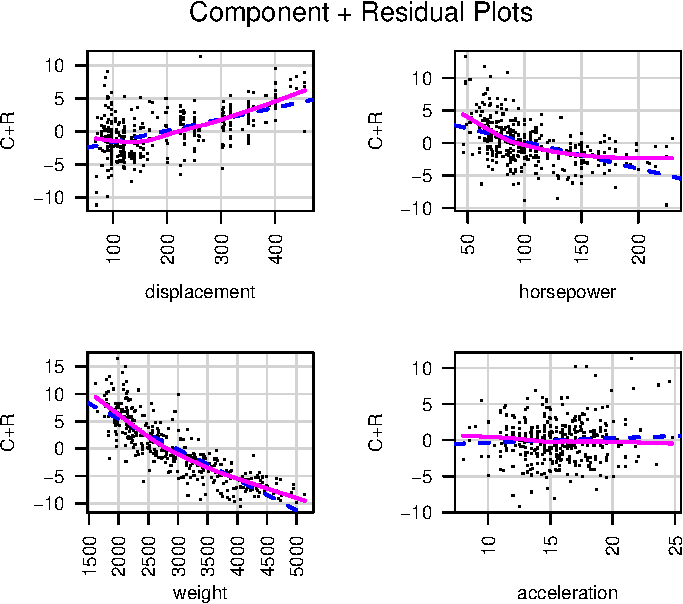
\includegraphics[width=0.7\linewidth]{Figures/Auto-explore-cr-plots-1}

}

\caption[Component + residual plots for the numeric predictors in the working model fit to the \code{Auto} data]{Component + residual plots for the numeric predictors in the working model fit to the \code{Auto} data.}\label{fig:Auto-explore-cr-plots}
\end{figure}
\end{CodeChunk}

The component + residual (``C+R'') plots in Figure
\ref{fig:Auto-explore-cr-plots}, produced by the \code{crPlots()}
function in the \pkg{car} package, clearly reveal the inadequacy of the
model. The broken blue lines in the C+R plots show linear least-squares
fits, while the solid magenta lines are nonparametric-regression
smooths.

Some background: As \citet[Sec.~8.2]{Weisberg:2014} explains, there are
technical advantages to having (numeric) predictors in linear regression
analysis that are themselves linearly related. If the predictors
\emph{aren't} linearly related, then the relationships between them can
often be straightened by power transformations. Transformations can be
selected after graphical examination of the data, or by analytic
methods, such as transforming the predictors towards multivariate
normality, which implies linearity. Once the relationships between the
predictors are linearized, it can be advantageous similarly to transform
the conditional distribution of the response variable towards normality.
Selecting transformations analytically raises the possibility of
automating the process, as required for cross-validation.

The \code{powerTransform()} function in the \pkg{car} package transforms
variables towards multivariate normality by a generalization of Box and
Cox's maximum-likelihood-like approach \citep{BoxCox:1964}. Although the
multinormal likelihood is maximized, the variables are transformed
individually. Several ``families'' of power transformations can be used,
including the original Box-Cox family (which is the default), simple
powers (and roots), and two adaptations of the Box-Cox family to data
that may include negative values and zeros: the Box-Cox-with-negatives
family and the Yeo-Johnson family; see \citet[Chap.~8]{Weisberg:2014}
and \citet[Chap.~3]{FoxWeisberg:2019} for details. We proceed to
transform the numeric predictors in the \code{Auto} regression towards
multivariate normality:

\begin{CodeChunk}
\begin{CodeInput}
R> num.predictors <- c("displacement", "horsepower", "weight",
+                     "acceleration")
R> tr.x <- powerTransform(Auto[, num.predictors])
R> summary(tr.x)
\end{CodeInput}
\begin{CodeOutput}
bcPower Transformations to Multinormality
             Est Power Rounded Pwr Wald Lwr Bnd Wald Upr Bnd
displacement   -0.0509           0      -0.2082       0.1065
horsepower     -0.1249           0      -0.2693       0.0194
weight         -0.0870           0      -0.2948       0.1208
acceleration    0.3061           0      -0.0255       0.6376

Likelihood ratio test that transformation parameters are equal to 0
 (all log transformations)
                               LRT df  pval
LR test, lambda = (0 0 0 0) 4.8729  4 0.301

Likelihood ratio test that no transformations are needed
                               LRT df   pval
LR test, lambda = (1 1 1 1) 390.08  4 <2e-16
\end{CodeOutput}
\end{CodeChunk}

We then apply the (rounded) transformations---all, as it turns out, logs
(i.e., ``zeroth'' powers)---to the data and re-estimate the model:

\begin{CodeChunk}
\begin{CodeInput}
R> A <- Auto
R> powers <- tr.x$roundlam
R> for (pred in num.predictors){
+   A[, pred] <- bcPower(A[, pred], lambda = powers[pred])
+ }
R> m <- update(m.auto, data = A)
\end{CodeInput}
\end{CodeChunk}

Having transformed the predictors towards multivariate normality, we now
consider whether there's evidence for transforming the response (using
\code{powerTransform()} for Box and Cox's original method), also
obtaining a log transformation:

\begin{CodeChunk}
\begin{CodeInput}
R> summary(powerTransform(m))
\end{CodeInput}
\begin{CodeOutput}
bcPower Transformation to Normality
   Est Power Rounded Pwr Wald Lwr Bnd Wald Upr Bnd
Y1    0.0024           0      -0.1607       0.1654

Likelihood ratio test that transformation parameter is equal to 0
 (log transformation)
                             LRT df  pval
LR test, lambda = (0) 0.00080154  1 0.977

Likelihood ratio test that no transformation is needed
                         LRT df   pval
LR test, lambda = (1) 124.13  1 <2e-16
\end{CodeOutput}
\begin{CodeInput}
R> m <- update(m, log(mpg) ~ .)
\end{CodeInput}
\end{CodeChunk}

The transformed numeric variables are much better-behaved and the
partial relationships in the model fit to the transformed data are much
more nearly linear (as we invite the reader to verify by redrawing the
scatterplot matrix for the transformed variables and the C+R plots for
the regression fit to the transformed data).

After transforming both the numeric predictors and the response, we
proceed to use the \code{stepAIC()} function in the \pkg{MASS} package
to perform predictor selection, employing the BIC model-selection
criterion (by setting the \code{k} argument of \code{stepAIC()} to
\(\log n\)):

\begin{CodeChunk}
\begin{CodeInput}
R> library("MASS")
R> m.step <- stepAIC(m, k = log(nrow(A)), trace = FALSE)
R> brief(m.step)
\end{CodeInput}
\begin{CodeOutput}
           (Intercept) horsepower weight acceleration year71   year72  year73
Estimate         9.435    -0.2763 -0.609      -0.1314 0.0280 -0.00711 -0.0395
Std. Error       0.262     0.0561  0.056       0.0532 0.0289  0.02845  0.0260
           year74 year75 year76 year77 year78 year79 year80 year81 year82
Estimate   0.0528 0.0532 0.0743 0.1379 0.1459 0.2360 0.3353 0.2629 0.3234
Std. Error 0.0300 0.0293 0.0282 0.0289 0.0275 0.0291 0.0311 0.0306 0.0296
           originEurope originJapan
Estimate         0.0558      0.0436
Std. Error       0.0168      0.0175

 Residual SD = 0.105 on 374 df, R-squared = 0.909
\end{CodeOutput}
\end{CodeChunk}

The selected model includes three of the numeric predictors,
\code{horsepower}, \code{weight}, and \code{acceleration}, along with
the factors \code{year} and \code{origin}. We can calculate the MSE for
this model, but we expect that the result will be optimistic because we
used the whole data to help specify the model:

\begin{CodeChunk}
\begin{CodeInput}
R> mse(Auto$mpg, exp(fitted(m.step)))
\end{CodeInput}
\begin{CodeOutput}
[1] 6.5121
attr(,"casewise loss")
[1] "(y - yhat)^2"
\end{CodeOutput}
\end{CodeChunk}

This is considerably smaller than the MSE for the original working
model:

\begin{CodeChunk}
\begin{CodeInput}
R> mse(Auto$mpg, fitted(m.auto))
\end{CodeInput}
\begin{CodeOutput}
[1] 8.0932
attr(,"casewise loss")
[1] "(y - yhat)^2"
\end{CodeOutput}
\end{CodeChunk}

A perhaps subtle point is that we compute the MSE for the selected model
on the original \code{mpg} response scale rather than the log scale, so
as to make the selected model comparable to the working
model.\footnote{That's slightly uncomfortable given the skewed
  distribution of \code{mpg}. An alternative is to use a robust measure
  of model lack-of-fit, such as the median absolute error instead of the
  mean-squared error, employing the \code{medAbsErr()} function from the
  \pkg{cv} package. The median absolute error, however, cannot be
  expressed as a casewise average (see Appendix A.2). Yet another
  possibility, suggested to us by a reviewer of an earlier version of
  this paper, is to compute the MSE for both models on the log-response
  scale rather than on the original scale of the response. This
  suggestion is quite general, in that the essential point is to use the
  \emph{same} response scale for all models to be compared, not
  necessarilty the \emph{original} scale of the response.}

The \code{"function"} method for \code{cv()} allows us to cross-validate
the whole model-selection procedure. The first argument to
\code{cv()}---here \code{selectTransStepAIC}---is a model-selection
function capable of refitting the model with a fold omitted and
returning a CV criterion:

\begin{CodeChunk}
\begin{CodeInput}
R> num.predictors
\end{CodeInput}
\begin{CodeOutput}
[1] "displacement" "horsepower"   "weight"       "acceleration"
\end{CodeOutput}
\begin{CodeInput}
R> cvs <- cv(selectTransStepAIC, data = Auto, seed = 76692,
+           working.model = m.auto, predictors = num.predictors,
+           response = "mpg", AIC = FALSE)
\end{CodeInput}
\begin{CodeOutput}
R RNG seed set to 76692
\end{CodeOutput}
\begin{CodeInput}
R> summary(cvs)
\end{CodeInput}
\begin{CodeOutput}
10-Fold Cross Validation
criterion: mse
cross-validation criterion = 7.4856
bias-adjusted cross-validation criterion = 7.3435
full-sample criterion = 6.5121
\end{CodeOutput}
\end{CodeChunk}

The other arguments to \code{cv()} are:\footnote{See \code{?cv.function}
  for additional optional arguments and details.}

\begin{itemize}
\tightlist
\item
  \code{data}, the data set to which the model is fit.
\item
  \code{seed}, an optional seed for \proglang{R}'s pseudo-random-number
  generator; as for \code{cv()}, if the seed isn't supplied by the user,
  then a seed is randomly selected and saved.
\item
  Arguments required by the model-selection function: the starting
  \code{working.model} (here, \code{m.auto}) for transformation and
  predictor selection; the names of the variables---\code{predictors}
  and \code{response}---that are candidates for transformation; and
  \code{AIC = FALSE}, which specifies use of the BIC for model
  selection.
\end{itemize}

Some noteworthy points:

\begin{itemize}
\tightlist
\item
  \code{selectTransStepAIC()} automatically computes CV cost criteria,
  here the MSE, on the \emph{untransformed} response scale.
\item
  As we anticipated, the estimate of the MSE that we obtain by
  cross-validating the whole model-specification process is larger than
  the MSE computed for the model we fit to the \code{Auto} data
  separately selecting transformations of the predictors and the
  response and then selecting predictors for the whole data set.
\item
  When we look at the transformations and predictors selected with each
  of the 10 folds omitted (i.e., the output of \code{compareFolds(cvs)},
  which isn't shown), we see that there is little uncertainty in
  choosing variable transformations, but considerably more uncertainty
  in subsequently selecting predictors: \code{horsepower},
  \code{weight}, and \code{year} are always included among the selected
  predictors; \code{acceleration} and \code{displacement} are included
  respectively in 4 and 3 of 10 selected models; and \code{cylinders}
  and \code{origin} are each included in only 1 of 10 models. Recall
  that when we selected predictors for the full data, we obtained a
  model with \code{horsepower}, \code{weight}, \code{acceleration},
  \code{year}, and \code{origin}.
\end{itemize}

\subsection[Example: Applying meta CV to polynomial regression for the
Auto data]{\texorpdfstring{Example: Applying meta CV to polynomial
regression for the \code{Auto}
data\footnote{What we call here ``meta CV'' has also been termed
  ``nested CV'' \citep[e.g., in the \pkg{cvms} package
  by][]{OlsenZachariae:2024}. We prefer, however, to reserve the term
  ``nested CV'' for the procedure described by
  \citet{BatesHastieTibshirani:2023}.}}{Example: Applying meta CV to polynomial regression for the Auto data}}\label{example-applying-meta-cv-to-polynomial-regression-for-the-auto-datameta-cv}

In Section~\ref{comparing-competing-models}, following \citet[Secs. 5.1,
5.3]{JamesEtAl:2021}, we fit polynomial regressions up to degree 10 to
the relationship of \code{mpg} to \code{horsepower} for the \code{Auto}
data, saving the 10 models, named \code{m.1} through \code{m.10}, in the
object \code{mlist}. We then used \code{cv()} to compare the
cross-validated MSE for the 10 models, discovering that the 7th degree
polynomial had the smallest MSE (by a small margin).

If we select the 7th degree polynomial model, intending to use it for
prediction, the CV estimate of the MSE for this model will be
optimistic. One solution is to cross-validate the process of using CV to
select the ``best'' model---that is, to apply meta-CV. The function
\code{selectModelList()}, which is suitable for use with \code{cv()},
implements this idea.

Applying \code{selectModelList()} to the \code{Auto}
polynomial-regression models, and using 10-fold CV, we
obtain:\footnote{Two functions are employed to access information in
  objects produced by functions in the \pkg{cv} package: \code{cvInfo()}
  and \code{as.data.frame()} are generic functions (the latter a
  standard-\proglang{R} generic) with methods for classes \code{"cv"},
  \code{"cvList"}, \code{"cvModlist"}, and \code{"cvSelect"} (in the
  case of \code{cvInfo()}) , and \code{"cv"}, \code{"cvList"}, and
  \code{"cvModlist"} (in the case of \code{as.data.frame()}). Here we
  use \code{cvInfo(metaCV.auto, "selected model")} to retrieve the model
  selected by \code{cv()} via \code{selectModelList()}. See \code{?cv}
  and \code{?cvInfo.cvSelect} for details.}

\begin{CodeChunk}
\begin{CodeInput}
R> metaCV.auto <- cv(selectModelList, data = Auto,
+                   working.model = mlist, save.model = TRUE,
+                        seed = 2120)
\end{CodeInput}
\begin{CodeOutput}
R RNG seed set to 2120
\end{CodeOutput}
\begin{CodeInput}
R> summary(metaCV.auto)
\end{CodeInput}
\begin{CodeOutput}
10-Fold Cross Validation
criterion: mse
cross-validation criterion = 20.012
bias-adjusted cross-validation criterion = 20.619
full-sample criterion = 18.746
\end{CodeOutput}
\begin{CodeInput}
R> brief(m.sel <- cvInfo(metaCV.auto, "selected model"))
\end{CodeInput}
\begin{CodeOutput}
           (Intercept) poly(horsepower, p)1 poly(horsepower, p)2
Estimate        23.446               -120.1                 44.1
Std. Error       0.217                  4.3                  4.3
           poly(horsepower, p)3 poly(horsepower, p)4 poly(horsepower, p)5
Estimate                  -3.95                -5.19                 13.3
Std. Error                 4.30                 4.30                  4.3
           poly(horsepower, p)6 poly(horsepower, p)7
Estimate                  -8.55                 7.98
Std. Error                 4.30                 4.30

 Residual SD = 4.3 on 384 df, R-squared = 0.702
\end{CodeOutput}
\begin{CodeInput}
R> cv(m.sel, seed = 2120)
\end{CodeInput}
\begin{CodeOutput}
R RNG seed set to 2120
\end{CodeOutput}
\begin{CodeOutput}
cross-validation criterion (mse) = 18.898
\end{CodeOutput}
\end{CodeChunk}

As expected, meta CV produces a larger estimate of MSE for the selected
7th degree polynomial model than CV applied directly to this model
(using the same seed for \proglang{R}'s random-number generator to
obtain the same folds).

We can equivalently call \code{cv()} with the list of models as its
first argument and set the argument \code{meta = TRUE} (identical output
not shown):

\begin{CodeChunk}
\begin{CodeInput}
R> summary(cv(mlist, data = Auto, seed = 2120, meta = TRUE,
+            save.model = TRUE))
\end{CodeInput}
\end{CodeChunk}

\section{Extending the cv package}\label{extending-the-cv-package}

The \pkg{cv} package is designed to be extensible in several directions.
In order of increasing general complexity, we can add: (1) a
cross-validation cost criterion; (2) a model class that's not directly
accommodated by the \code{cv()} default method or by another directly
inherited method; and (3) a new model-selection procedure suitable for
use with the \code{"function"} method for \code{cv()}. In this section,
we illustrate (1) and (2); more diverse and extensive examples
(including of (3)) may be found in the vignette on extending the
\pkg{cv} package.

Suppose that we want to cross-validate a multinomial logistic regression
model fit by the \code{multinom()} function in the \pkg{nnet} package
\citep{VenablesRipley:2002}. We borrow an example from \citet[Sec.~14.2.1]{Fox:2016},
with data from the British Election Panel Study on
vote choice in the 2001 UK election. Data for the example are in the
\code{BEPS} data set in the \pkg{carData} package:

\begin{CodeChunk}
\begin{CodeInput}
R> data("BEPS", package = "carData")
R> summary(BEPS)
\end{CodeInput}
\begin{CodeOutput}
               vote          age       economic.cond.national
 Conservative    :462   Min.   :24.0   Min.   :1.00
 Labour          :720   1st Qu.:41.0   1st Qu.:3.00
 Liberal Democrat:343   Median :53.0   Median :3.00
                        Mean   :54.2   Mean   :3.25
                        3rd Qu.:67.0   3rd Qu.:4.00
                        Max.   :93.0   Max.   :5.00
 economic.cond.household     Blair          Hague         Kennedy
 Min.   :1.00            Min.   :1.00   Min.   :1.00   Min.   :1.00
 1st Qu.:3.00            1st Qu.:2.00   1st Qu.:2.00   1st Qu.:2.00
 Median :3.00            Median :4.00   Median :2.00   Median :3.00
 Mean   :3.14            Mean   :3.33   Mean   :2.75   Mean   :3.14
 3rd Qu.:4.00            3rd Qu.:4.00   3rd Qu.:4.00   3rd Qu.:4.00
 Max.   :5.00            Max.   :5.00   Max.   :5.00   Max.   :5.00
     Europe      political.knowledge    gender
 Min.   : 1.00   Min.   :0.00        female:812
 1st Qu.: 4.00   1st Qu.:0.00        male  :713
 Median : 6.00   Median :2.00
 Mean   : 6.73   Mean   :1.54
 3rd Qu.:10.00   3rd Qu.:2.00
 Max.   :11.00   Max.   :3.00
\end{CodeOutput}
\end{CodeChunk}

The polytomous (multi-category) response variable is \code{vote}, a
factor with levels \code{"Conservative"}, \code{"Labour"}, and
\code{"Liberal Democrat"}. The predictors of \code{vote} are:

\begin{itemize}
\tightlist
\item
  \code{age}, in years.
\item
  \code{econ.cond.national} and \code{econ.cond.household}, the
  respondent's ratings of the state of the economy, on 1 to 5 scales.
\item
  \code{Blair}, \code{Hague}, and \code{Kennedy}, ratings of the leaders
  of the Labour, Conservative, and Liberal Democratic parties, on 1 to 5
  scales.
\item
  \code{Europe}, an 11-point scale for attitude towards European
  integration, with high scores representing ``Euro-skepticism.''
\item
  \code{political.knowledge}, knowledge of the parties' positions on
  European integration, with scores from 0 to 3.
\item
  \code{gender}, \code{"female"} or \code{"male"}.
\end{itemize}

The model fit to the data includes an interaction between \code{Europe}
and \code{political.knowledge}, which was the focus of the original
research on which this example is based
\citep{AndersenHeathSinnott:2002}; the other predictors enter the model
additively:

\begin{CodeChunk}
\begin{CodeInput}
R> library("nnet", quietly = TRUE)
R> m.beps <- multinom(vote ~ age + gender + economic.cond.national
+                         + economic.cond.household + Blair + Hague
+                         + Kennedy + Europe * political.knowledge,
+                    data = BEPS, trace = FALSE)
\end{CodeInput}
\end{CodeChunk}

Figure~\ref{fig:BEPS-plot} shows an ``effect plot,'' using the
\pkg{effects} package \citep{FoxWeisberg:2019} to visualize the
\code{Europe} \(\times\) \code{political.knowledge} interaction in a
``stacked-area'' graph:

\begin{CodeChunk}
\begin{CodeInput}
R> plot(effects::Effect(c("Europe", "political.knowledge"), m.beps,
+             xlevels = list(Europe = 1:11, political.knowledge = 0:3),
+             fixed.predictors = list(given.values = c(gendermale = 0.5))),
+      lines = list(col = c("blue", "red", "orange")),
+      axes = list(x = list(rug = FALSE), y = list(style = "stacked")))
\end{CodeInput}
\begin{figure}

{\centering 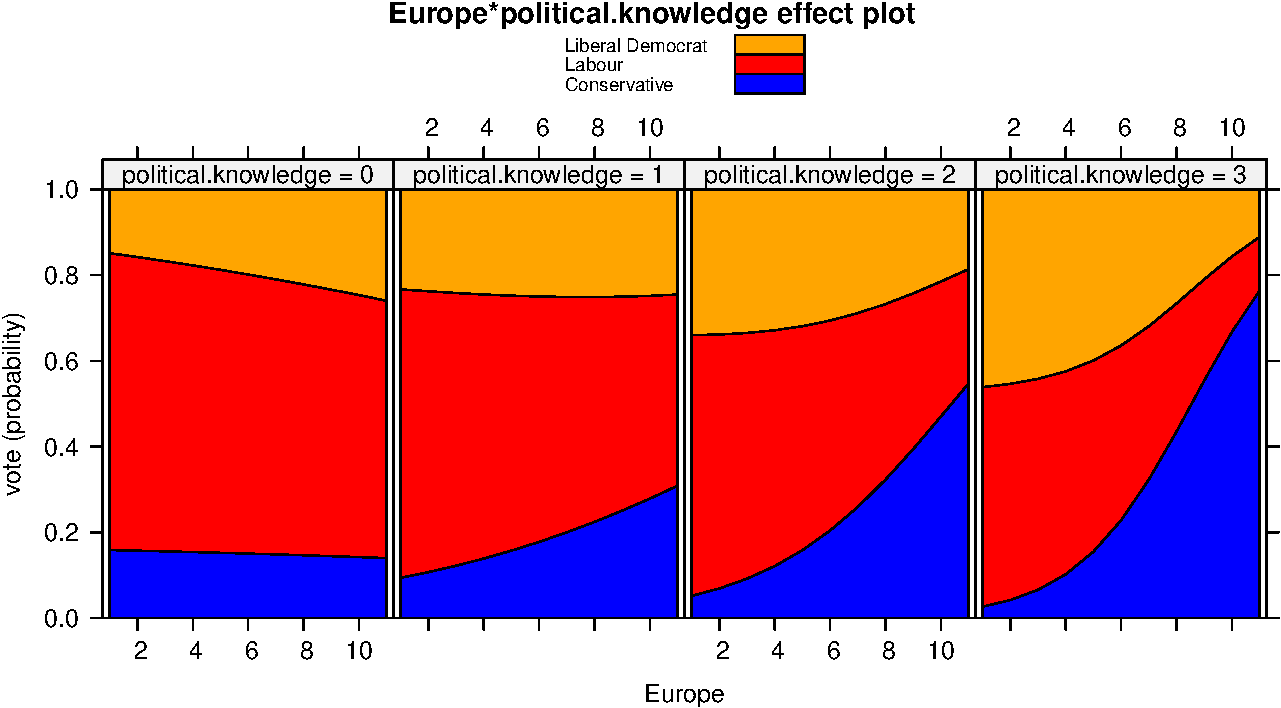
\includegraphics{Figures/BEPS-plot-1}

}

\caption[Effect plot for the interaction between attitude towards European integration and political knowledge in the multinomial logit model fit to voting data from the 2001 British Election Panel Study, using party colors]{Effect plot for the interaction between attitude towards European integration and political knowledge in the multinomial logit model fit to voting data from the 2001 British Election Panel Study, using party colors.}\label{fig:BEPS-plot}
\end{figure}
\end{CodeChunk}

As political knowledge increased, voters tended to align their votes
more closely with the party positions on European integration: The
Conservative Party was relatively Euro-skeptic, while Labour and the
Liberal Democrats were more supportive of the UK's participation in the
EU.

To cross-validate this multinomial-logit model we need an appropriate
cost criterion. None of the criteria in the \pkg{cv} package will
do---for example, \code{mse()} is appropriate only for a numeric
response. The \code{BayesRule()} criterion, also supplied by \pkg{cv},
which is for a binary response, comes close:

\begin{CodeChunk}
\begin{CodeInput}
R> BayesRule
\end{CodeInput}
\begin{CodeOutput}
function (y, yhat)
{
    if (!all(y %in% c(0, 1)))
        stop("response values not all 0 or 1")
    if (any(yhat < 0) || any(yhat > 1))
        stop("fitted values outside of interval [0, 1]")
    yhat <- round(yhat)
    result <- mean(y != yhat)
    attr(result, "casewise loss") <- "y != round(yhat)"
    result
}
<bytecode: 0x11188dee8>
<environment: namespace:cv>
\end{CodeOutput}
\end{CodeChunk}

After doing some error checking, \code{BayesRule()} rounds the predicted
probability \code{yhat} of a 1 (``success'') response in a binary
regression model to 0 or 1 to obtain a categorical prediction, and then
reports the proportion of incorrect predictions. Because the Bayes's
rule criterion is an average of casewise components (as, e.g., is the
MSE), a \code{"casewise loss"} attribute is attached to the result,
enabling the computation of bias correction and confidence intervals (as
discussed in Appendix A.2).

It is straightforward to adapt Bayes's rule to a polytomous response:

\begin{CodeChunk}
\begin{CodeInput}
R> head(BEPS$vote)
\end{CodeInput}
\begin{CodeOutput}
[1] Liberal Democrat Labour           Labour           Labour
[5] Labour           Labour
Levels: Conservative Labour Liberal Democrat
\end{CodeOutput}
\begin{CodeInput}
R> yhat <- predict(m.beps, type = "class")
R> head(yhat)
\end{CodeInput}
\begin{CodeOutput}
[1] Labour           Labour           Labour           Labour
[5] Liberal Democrat Labour
Levels: Conservative Labour Liberal Democrat
\end{CodeOutput}
\begin{CodeInput}
R> BayesRuleMulti <- function(y, yhat){
+   result <- mean(y != yhat)
+   attr(result, "casewise loss") <- "y != yhat"
+   result
+ }
R>
R> BayesRuleMulti(BEPS$vote, yhat)
\end{CodeInput}
\begin{CodeOutput}
[1] 0.31869
attr(,"casewise loss")
[1] "y != yhat"
\end{CodeOutput}
\end{CodeChunk}

The \code{predict()} method for \code{"multinom"} models called with
argument \code{type = "class"} reports the Bayes's rule prediction for
each case---that is, the response category with the highest predicted
probability. The argument \code{yhat} to our \code{BayesRuleMulti()}
function is the vector of Bayes's rule categorical predictions, while
\code{y} is the vector of observed categorical responses. The function
calculates and returns the proportion of misclassified cases. Because
this value is also the mean of casewise components, we attach a
\code{"casewise loss"} attribute to the result.

The marginal proportions for the response categories are

\begin{CodeChunk}
\begin{CodeInput}
R> xtabs(~ vote, data = BEPS) / nrow(BEPS)
\end{CodeInput}
\begin{CodeOutput}
vote
    Conservative           Labour Liberal Democrat
         0.30295          0.47213          0.22492
\end{CodeOutput}
\end{CodeChunk}

and so the marginal Bayes's rule prediction, that everyone will vote
Labour, produces an error rate of \(1 - 0.47213 = 0.52787\). The
multinomial-logit model appears to do substantially better than that,
but does its performance hold up to cross-validation?

We check first whether the default \code{cv()} method works
``out-of-the-box'' for the \code{"multinom"} model:

\begin{CodeChunk}
\begin{CodeInput}
R> cv(m.beps, seed = 3465, criterion = BayesRuleMulti)
\end{CodeInput}
\begin{CodeOutput}
Error in GetResponse.default(model): non-vector response
\end{CodeOutput}
\end{CodeChunk}

The default method of \code{GetResponse()} (a function supplied by the
\pkg{cv} package---see \code{?GetResponse}) fails for a
\code{"multinom"} object. A straightforward solution is to supply a
\code{GetResponse.multinom()} method that returns the factor response
{[}using the \code{get\_response()} function from the \pkg{insight}
package,

\begin{CodeChunk}
\begin{CodeInput}
R> GetResponse.multinom <- function(model, ...) {
+   insight::get_response(model)
+ }
R>
R> head(GetResponse(m.beps))
\end{CodeInput}
\begin{CodeOutput}
[1] Liberal Democrat Labour           Labour           Labour
[5] Labour           Labour
Levels: Conservative Labour Liberal Democrat
\end{CodeOutput}
\end{CodeChunk}

and to try again:

\begin{CodeChunk}
\begin{CodeInput}
R> cv(m.beps, seed = 3465, criterion = BayesRuleMulti)
\end{CodeInput}
\begin{CodeOutput}
R RNG seed set to 3465
\end{CodeOutput}
\begin{CodeOutput}
Error in match.arg(type): 'arg' should be one of "class", "probs"
\end{CodeOutput}
\end{CodeChunk}

A \code{traceback()} (not shown) reveals that the problem is that the
default method of \code{cv()} calls the \code{"multinom"} method for
\code{predict()} with the argument \code{type="response"}, when the
correct argument should be \code{type="class"}. We therefore must write
a \code{"multinom"} method for \code{cv()}, but that proves to be very
simple:

\begin{CodeChunk}
\begin{CodeInput}
R> cv.multinom <- function (model, data, criterion = BayesRuleMulti,
+                          k, reps, seed, ...) {
+     model <- update(model, trace = FALSE)
+     NextMethod(
+       type = "class", criterion = criterion,
+       criterion.name = deparse(substitute(criterion))
+     )
+   }
\end{CodeInput}
\end{CodeChunk}

That is, we simply call the default \code{cv()} method (via
\code{NextMethod()}) with the \code{type} argument properly set. In
addition to supplying the correct \code{type} argument, our method sets
the default \code{criterion} for the \code{cv.multinom()} method to
\code{BayesRuleMulti}. Adding the argument
\code{criterion.name = deparse(substitute(criterion))} is inessential,
but it insures that printed output will include the name of the
criterion function that's employed, whether it's the default
\code{BayesRuleMulti} or something else. Prior to invoking
\code{NextMethod()}, we call \code{update()} with \code{trace = FALSE}
to suppress the iteration history reported by default by
\code{multinom()}---it would be tedious to see the iteration history for
each fold.

Then:

\begin{CodeChunk}
\begin{CodeInput}
R> summary(cv(m.beps, seed = 3465))
\end{CodeInput}
\begin{CodeOutput}
R RNG seed set to 3465
\end{CodeOutput}
\begin{CodeOutput}
10-Fold Cross Validation
criterion: BayesRuleMulti
cross-validation criterion = 0.32459
bias-adjusted cross-validation criterion = 0.32368
95% CI for bias-adjusted CV criterion = (0.30017, 0.34718)
full-sample criterion = 0.31869
\end{CodeOutput}
\end{CodeChunk}

The cross-validated polytomous Bayes's rule criterion confirms that the
fitted model does substantially better than the marginal Bayes's rule
prediction that everyone votes for Labour.

\section{Comparing cv to other software for
cross-validation}\label{comparing-cv-to-other-software-for-cross-validation}

In this section with briefly compare the \code{cv} package to other
packages in \proglang{R} that support cross-validation, and then even
more briefly consider facilities for cross-validation in other commonly
used statistical software, \proglang{SAS}, \proglang{Stata}, and
\proglang{Python}.

\subsection[Other R software]{Other \proglang{R} software}\label{other-r-software}

The \pkg{cv} package is far from unique in implementing cross-validation
of regression models in \proglang{R}. We've already mentioned the
\code{cv.glm()} function in the \pkg{boot} package. A general review of
CV facilities in \proglang{R} is beyond the scope of the current paper,
but in this section we remark selectively on other \proglang{R} packages
that support CV.

Our goal in implementing CV is to make it conveniently available to
\proglang{R} users with limited programming skills,\footnote{\proglang{R}
  users with sophisticated programming skills would generally find it
  unchallenging to implement CV directly for specific applications (as
  we illustrate below). Even in this case, however, there's an argument
  for using a simple pre-programmed interface to CV, to minimize
  programming effort and to avoid mistakes.} and hence to encourage its
use. Towards this end, the \pkg{cv} package provides a simple,
consistent interface through the \code{cv()} generic function, with
specific methods for different classes of standard \proglang{R}
statistical models. Moreover, we have tried to make writing methods for
additional classes of statistical models as simple and straightforward
as possible. Because CV is computationally intensive, we also aim for
efficiency, by enabling parallel computations generally, and by
exploiting properties of specific classes of statistical models (in
particular, computations based on hatvalues and the Woodbury matrix
identity for linear and generalized linear model). Finally, the package
includes some unusual features, such as general support for
mixed-effects models and for cross-validating complex
model-specification procedures.

Some \proglang{R} packages for statistical learning include facilities
for cross-validation. Notable examples are the \pkg{caret} package
\citep{Kuhn:2008} and the \pkg{tidyfit} package \citep{Pfitzinger:2024};
the latter employs \pkg{rsample} \citep{FrickEtAl:2024} for CV, which we
will discuss presently. This contrasts with the approach taken in the
\pkg{cv} package, which, as we have explained, directly supports classes
of standard \proglang{R} statistical models.

Other packages, including \pkg{cvms} \citep{OlsenZachariae:2024},
\pkg{mlexperiments} \citep{Kapsner:2024}, \pkg{origami}
\citep{CoyleEtAl:2022}, and \pkg{rsample} (which also implements
bootstrapping), modularize the CV process to a greater or lesser extent.
Advantages of this approach include flexibility and generality, but a
disadvantage is that use of these packages entails nontrivial
programming effort and skill.

We illustrate with an example adapted from a vignette in the
\pkg{rsample} package, which uses the \code{attrition} data set from the
\pkg{modeldata} package \citep{Kuhn:2024}, comparing LOO CV computed
using the \code{cv()} function in the \pkg{cv} package to LOO CV
computed using the \pkg{caret} and \pkg{rsample} packages. At more than
15 million cumulative downloads, \pkg{caret} is by a very wide margin
the most downloaded from the RStudio CRAN mirror of the \proglang{R}
packages mentioned above. Among the packages that focus more on
cross-validation, \pkg{rsample} is the most downloaded, at nearly 4
million downloads.

Here, with minimal explanation, is how one would perform LOO CV for this
example using \pkg{rsample}:\footnote{The example in the \pkg{rsample}
  vignette uses 10-fold rather than LOO CV, but otherwise the code from
  the vignette is only trivially modified here.}

\begin{CodeChunk}
\begin{CodeInput}
R> library("rsample")
R>
R> data("attrition", package = "modeldata")
R> nrow(attrition)
\end{CodeInput}
\begin{CodeOutput}
[1] 1470
\end{CodeOutput}
\begin{CodeInput}
R> mod_form <- Attrition ~ JobSatisfaction + Gender + MonthlyIncome
R>
R> rs_obj <- loo_cv(attrition)
R>
R> holdout_results <- function(splits, ...) {
+   mod <- glm(..., data = analysis(splits), family = binomial)
+   holdout <- assessment(splits)
+   res <- broom::augment(mod, newdata = holdout)
+   lvls <- levels(holdout$Attrition)
+   predictions <- factor(ifelse(res$.fitted > 0, lvls[2], lvls[1]),
+                         levels=lvls)
+   res$correct <- predictions == holdout$Attrition
+   res
+ }
R>
R> library("purrr", warn.conflicts=FALSE)
R>
R> rs_obj$results <- map(rs_obj$splits, holdout_results, mod_form)
R> rs_obj$accuracy <- map_dbl(rs_obj$results, function(x) mean(x$correct))
R> 1 - summary(rs_obj$accuracy)
\end{CodeInput}
\begin{CodeOutput}
   Min. 1st Qu.  Median    Mean 3rd Qu.    Max.
  1.000   0.000   0.000   0.161   0.000   0.000
\end{CodeOutput}
\end{CodeChunk}

The response variable in this example, \code{Attrition}, is binary. The
function \code{holdout_results()} must be supplied by the user, and mean
``\code{accuracy}'' is the complement of the Bayes-rule classification
error rate.

In this case, it's simple (and, in our opinion, simpler) to program LOO
CV directly. For example,

\begin{CodeChunk}
\begin{CodeInput}
R> mod.attrition <- glm(mod_form, data = attrition, family = binomial)
R> n <- nrow(attrition)
R> yhat <- numeric(n)
R> for (i in 1:n){
+   m <- update(mod.attrition, data = attrition[-i, ])
+   yhat[i] <- predict(m, newdata = attrition[i, ], type = "response")
+ }
R> mean(((attrition$Attrition == "Yes") - round(yhat)) ^ 2)
\end{CodeInput}
\begin{CodeOutput}
[1] 0.16122
\end{CodeOutput}
\end{CodeChunk}

The \pkg{caret} package supports generalized linear models fit by
\code{glm()} and can straightforwardly perform LOO CV:

\begin{CodeChunk}
\begin{CodeInput}
R> library("ggplot2", warn.conflicts = FALSE)
R> library("caret", quietly = TRUE, warn.conflicts = FALSE)
R> train(x = attrition[, c("JobSatisfaction", "Gender", "MonthlyIncome")],
+       y = attrition$Attrition, method = "glm",
+       trControl = trainControl(method = "LOOCV"))
\end{CodeInput}
\begin{CodeOutput}
Generalized Linear Model

1470 samples
   3 predictor
   2 classes: 'No', 'Yes'

No pre-processing
Resampling: Leave-One-Out Cross-Validation
Summary of sample sizes: 1469, 1469, 1469, 1469, 1469, 1469, ...
Resampling results:

  Accuracy  Kappa
  0.83878   0
\end{CodeOutput}
\end{CodeChunk}

where ``\code{Accuracy},'' again, is the complement of the
misclassification rate.

And here's how we can perform the same computation using the \code{cv()}
function in the \pkg{cv} package:

\begin{CodeChunk}
\begin{CodeInput}
R> cv(mod.attrition, k = "loo", criterion = BayesRule)
\end{CodeInput}
\begin{CodeOutput}
cross-validation criterion (BayesRule) = 0.16122
\end{CodeOutput}
\begin{CodeInput}
R> 1 - mean(rs_obj$accuracy)
\end{CodeInput}
\begin{CodeOutput}
[1] 0.16122
\end{CodeOutput}
\end{CodeChunk}

Let's compare the computational efficiency of the various
implementations, also showing the use of \code{method = "Woodbury"} and
\code{method =" hatvalues"} for \code{cv()}, which, in this example,
produce numerically identical results to the default
\code{method = "exact"}:\footnote{As before, we ask
  \code{microbenchmark()} to report relative timings, and also as
  before, we set \code{times = 10} rather than the default
  \code{times = 100}.}

\begin{CodeChunk}
\begin{CodeInput}
R> set.seed(53437)
R> print(microbenchmark::microbenchmark(
+   cv.hatvalues = cv(mod.attrition, k = "loo", criterion = BayesRule,
+                     method = "hatvalues"),
+   cv.wood = cv(mod.attrition, k = "loo", criterion = BayesRule,
+                method = "Woodbury"),
+   cv.exact = cv(mod.attrition, k = "loo", criterion = BayesRule),
+   direct = {
+     n <- nrow(attrition)
+     yhat <- numeric(n)
+     for (i in 1:n){
+       m <- update(mod.attrition, data = attrition[-i, ])
+       yhat[i] <- predict(m, newdata = attrition[i, ], type = "response")
+     }
+     mean(((attrition$Attrition == "Yes") - round(yhat)) ^ 2)
+   },
+   rsample = {
+     rs_obj$results <- map(rs_obj$splits, holdout_results, mod_form)
+     rs_obj$accuracy <- map_dbl(rs_obj$results,
+                                function(x) mean(x$correct))
+   },
+   caret = train(x = attrition[, c("JobSatisfaction", "Gender",
+                                   "MonthlyIncome")],
+               y = attrition$Attrition,
+               method = "glm",
+               trControl = trainControl(method = "LOOCV")),
+   times = 10, unit = "relative"), signif = 3)
\end{CodeInput}
\begin{CodeOutput}
Warning in microbenchmark::microbenchmark(cv.hatvalues = cv(mod.attrition, :
less accurate nanosecond times to avoid potential integer overflows
\end{CodeOutput}
\begin{CodeOutput}
Unit: relative
         expr    min   lq   mean median     uq    max neval   cld
 cv.hatvalues    1.0    1    1.0    1.0    1.0    1.0    10 a
      cv.wood   50.4   46   47.5   48.5   46.1   47.2    10 a
     cv.exact 2240.0 2010 2000.0 1980.0 1900.0 1960.0    10  b
       direct 2500.0 2240 2200.0 2200.0 2100.0 2040.0    10   c
      rsample 2770.0 2510 2560.0 2460.0 2330.0 3100.0    10    d
        caret 3250.0 2930 2880.0 2870.0 2760.0 2710.0    10     e
\end{CodeOutput}
\end{CodeChunk}

Computing time for \pkg{rsample} and \pkg{caret} for this problem is
similar to direct computation of LOO CV and to \code{cv()} with
\code{method="exact"}, but almost two orders of magnitude slower than
\code{cv()} with \code{method="Woodbury"}, and more than three orders of
magnitude slower than \code{cv()} with \code{method="hatvalues"}.

\subsection[Comparing cv to other software for cross-validation: SAS,
Stata, and Python]
{Comparing cv to other software for cross-validation: \proglang{SAS},
\proglang{Stata}, and \proglang{Python}}
\label{comparing-cv-to-other-software-for-cross-validation-sas-stata-and-python}

Although we do not have recent experience with statistical software for
cross-validation other than in \proglang{R},\footnote{It is our
  impression that these three statistical systems, in addition to
  \proglang{R}, are most likely to be used for applications of
  cross-validation. We were once frequent users of \proglang{SAS},
  though not recently, and have only cursory experience with
  \proglang{Stata} and \proglang{Python}, so we are not ideally situated
  to evaluate CV software for any of the three.} we have examined
provisions for CV in \proglang{SAS}, \proglang{Stata}, and
\proglang{Python}, primarily by locating and reading documentation.

\subsubsection[SAS]{\proglang{SAS}}\label{sas}

Cross-validation in \proglang{SAS} is associated with particular
procedures (``\code{PROC}s''), and is distributed across several
products, including, for example, \code{PROC LOGISTIC} and
\code{PROC PLS} in \proglang{SAS/STAT} \citep{SAS-Stat:2020}, in
\proglang{SAS Enterprise Miner} \citep{SAS-Enterprise-Miner:2018}, and
in \proglang{SAS Visual Data Mining and Machine Learning}
\citep{SAS-Visual-Data-Mining:2020}. These appear to be straightforward
implementations of \(k\)-fold CV.

In addition, \proglang{SAS} has programming capabilities, including via
its macro language, and we're aware of several independent
implementations of CV in \proglang{SAS} macros. These tend to be limited
in scope. For example \citet{Slaets-et-al:2014} employ and provide
access to a \proglang{SAS} macro for \(k\)-fold CV of mixed-effects
models, which repeatedly calls \code{PROC MIXED} in \proglang{SAS/STAT},
and which performs cluster-based resampling (one of the options that we
provide for mixed-effects models in the \pkg{cv} package).

\subsubsection[Stata]{\proglang{Stata}}\label{stata}

As far as we can tell, \proglang{Stata} has no standard implementation
of cross-validation. Like \proglang{R}, however, \proglang{Stata} is
extensible through a programming language that allows users to define
new commands in so-called ``\code{ado}'' files.

Several such contributed \proglang{Stata} CV commands, varying in
generality, are shared in an archive maintained at the Boston College
Department of Economics. For example, the \code{CV\_REGRESS} command
\citep{Rios-Avila:2018} computes leave-one-out CV for least-squares
regression using the hatvalues, and thus is comparable to \code{cv()}
for linear models with \code{method = "hatvalues"}. In contrast, the
\code{CROSSVALIDATE} command \citep{Schonlau:2020} performs \(k\)-fold
CV for a wide range of regression models fit in \proglang{Stata}, and is
roughly comparable to the default method of \code{cv()}, although
\code{CROSSVALIDATE} returns cross-validated fitted values, from which
cost criteria can be computed, rather than (as \code{cv()})
cost-criteria directly.

\subsubsection[Python]{\proglang{Python}}\label{python}

The programming language \proglang{Python} is often the software of
choice for ``machine learning,'' in which cross-validation can play a
prominent role. Machine learning and statistical modeling more generally
are supported through extensive \proglang{Python} libraries, such as
\pkg{scikit-learn}
\citep{Pedregosa-et-al:2011, ScikitLearnDevelopers:2024} and
\pkg{TensorFlow} \citep[which isn't limited to use within
\proglang{Python}]{TensorFlow:2015}.

Functions for cross-validation are provided in \pkg{scikit-learn}, which
supports \(k\)-fold, repeated \(k\)-fold, and leave-one-out CV. These
functions can be applied to data sets consisting of independent
observations, hierarchical groups, or time-series data. A sample program
in the \pkg{scikit-learn} documentation
\citep{ScikitLearnDevelopers:2024} demonstrates how to implement meta
cross-validation (termed ``nested cross-validation'' in the
documentation).

The approach taken by \pkg{scikit-learn} for independent observations is
similar to that in the default \code{cv()} method in the \pkg{cv}
package. The approach for hierarchical data is similar, but not
identical, to that in \pkg{cv} (as described in Section
\ref{cross-validating-mixed-effects-models}). Our \pkg{cv} package
doesn't currently provide for cross-validating time-series models, but
we anticipate that a future version of the package will.

\section*{Appendix: Computational
notes}\label{appendix-computational-notes}
\addcontentsline{toc}{section}{Appendix: Computational notes}

\subsection*{A.1 Efficient computations for linear and generalized
linear
models}\label{a.1-efficient-computations-for-linear-and-generalized-linear-models}
\addcontentsline{toc}{subsection}{A.1 Efficient computations for linear
and generalized linear models}

The most straightforward way to implement cross-validation in
\proglang{R} for statistical modeling functions that are written in the
canonical manner is to use \code{update()} to refit the model with each
fold removed. This is the approach taken in the default method for
\code{cv()}, and it is appropriate if the cases are independently
sampled. Refitting the model in this manner for each fold is generally
feasible when the number of folds is modest, but can be prohibitively
costly for leave-one-out cross-validation when the number of cases is
large.

The \code{"lm"} and \code{"glm"} methods for \code{cv()} take advantage
of computational efficiencies by avoiding refitting the model with each
fold removed. Consider, in particular, the weighted linear model
\(\mathbf{y}_{n \times 1} = \mathbf{X}_{n \times p}\boldsymbol{\beta}_{p \times 1} + \boldsymbol{\varepsilon}_{n \times 1}\),
where
\(\boldsymbol{\varepsilon} \sim \mathbf{N}_n \left(\mathbf{0}, \sigma^2 \mathbf{W}^{-1}_{n \times n}\right)\).
Here, \(\mathbf{y}\) is the response vector, \(\mathbf{X}\) the model
matrix, and \(\boldsymbol{\varepsilon}\) the error vector, each for
\(n\) cases, and \(\boldsymbol{\beta}\) is the vector of \(p\)
population regression coefficients. The errors are assumed to be
multivariately normally distributed with 0 means and covariance matrix
\(\sigma^2 \mathbf{W}^{-1}\), where \(\mathbf{W} = \mathrm{diag}(w_i)\)
is a diagonal matrix of inverse-variance weights. For the linear model
with constant error variance, the weight matrix is taken to be
\(\mathbf{W} = \mathbf{I}_n\), the order-\(n\) identity matrix.

The weighted-least-squares (``WLS'') estimator of \(\boldsymbol{\beta}\)
is \citep[see, e.g.,][Sec.~12.2.2]{Fox:2016} \footnote{This is a
  definitional formula, which assumes that the model matrix
  \(\mathbf{X}\) is of full column rank, and which can be subject to
  numerical instability when \(\mathbf{X}\) is ill-conditioned.
  \code{lm()} uses the QR decomposition of the model matrix with
  pivoting to obtain computationally more stable results.} \[
\mathbf{b}_{\mathrm{WLS}} = \left( \mathbf{X}^\top \mathbf{W} \mathbf{X} \right)^{-1}
  \mathbf{X}^\top \mathbf{W} \mathbf{y}
\]

Fitted values are then
\(\widehat{\mathbf{y}} = \mathbf{X}\mathbf{b}_{\mathrm{WLS}}\).

The LOO fitted value for the \(i\)th case can be efficiently computed by
\(\widehat{y}_{-i} = y_i - e_i/(1 - h_i)\) where
\(h_i = \mathbf{x}^\top_i \left( \mathbf{X}^\top \mathbf{W} \mathbf{X} \right)^{-1} \mathbf{x}_i\)
(the so-called ``hatvalue''). Here, \(\mathbf{x}^\top_i\) is the \(i\)th
row of \(\mathbf{X}\), and \(\mathbf{x}_i\) is the \(i\)th row written
as a column vector. This approach can break down when one or more
hatvalues are equal to 1, in which case the formula for
\(\widehat{y}_{-i}\) requires division by 0. Then the ``training'' set
omitting the observation with hatvalue = 1 is rank-deficient and the
predictors for the left-out case are outside the linear span of the
predictors in the training set.

To compute cross-validated fitted values when the folds contain more
than one case, we make use of the Woodbury matrix identity
\citep{Hager:1989}, \[
\left(\mathbf{A}_{m \times m} + \mathbf{U}_{m \times k}
\mathbf{C}_{k \times k} \mathbf{V}_{k \times m} \right)^{-1} = \mathbf{A}^{-1} - \mathbf{A}^{-1}\mathbf{U} \left(\mathbf{C}^{-1} +
\mathbf{VA}^{-1}\mathbf{U} \right)^{-1} \mathbf{VA}^{-1}
\] where \(\mathbf{A}\) is a nonsingular order-\(m\) matrix. We apply
this result by letting \begin{align*}
    \mathbf{A} &= \mathbf{X}^\top \mathbf{W} \mathbf{X} \\
    \mathbf{U} &= \mathbf{X}_\mathbf{j}^\top \\
    \mathbf{V} &= - \mathbf{X}_\mathbf{j} \\
    \mathbf{C} &= \mathbf{W}_\mathbf{j} \\
\end{align*} where the subscript
\(\mathbf{j} = (i_{j1}, \ldots, i_{jm})^\top\) represents the vector of
indices for the \(m = n_j \approx n/k\) cases in the \(j\)th fold. The
negative sign in \(\mathbf{V} = - \mathbf{X}_\mathbf{j}\) reflects the
\emph{removal}, rather than addition, of the cases in \(\mathbf{j}\).

Applying the Woodbury identity isn't quite as fast as using the
hatvalues, but it is generally much faster than refitting the model. A
disadvantage of the Woodbury identity, however, is that it entails
explicit matrix inversion and thus may be numerically unstable. The
inverse of \(\mathbf{A} = \mathbf{X}^\top \mathbf{W} \mathbf{X}\) is
available directly in the \code{"lm"} object, but the second term on the
right-hand side of the Woodbury identity requires a matrix inversion
with each fold deleted. (In contrast, the inverse of each
\(\mathbf{C} = \mathbf{W}_\mathbf{j}\) is straightforward because
\(\mathbf{W}\) is diagonal.)

The Woodbury identity also requires that the model matrix be of full
rank. We impose that restriction in our code by removing redundant
regressors from the model matrix for all of the cases, but that doesn't
preclude rank deficiency from surfacing when a fold is removed. Rank
deficiency of \(\mathbf{X}\) doesn't disqualify cross-validation because
all we need are fitted values under the estimated model.

\code{glm()} computes the maximum-likelihood estimates for a generalized
linear model by iterated weighted least squares \citep[see, e.g.,][Sec.~6.12]{FoxWeisberg:2019}.
The last iteration is therefore just a WLS fit
of the ``working response'' on the model matrix using ``working
weights.'' Both the working weights and the working response at
convergence are available from the information in the object returned by
\code{glm()}.

We then treat re-estimation of the model with a case or cases deleted as
a WLS problem, using the hatvalues or the Woodbury matrix identity. The
resulting fitted values for the deleted fold aren't exact---that is,
except for the Gaussian family, the result isn't identical to what we
would obtain by literally refitting the model---but in our (limited)
experience, the approximation is very good, especially for LOO CV, which
is when we would be most tempted to use it. Nevertheless, because these
results are approximate, the default for the \code{"glm"} \code{cv()}
method is to perform the exact computation, which entails refitting the
model with each fold omitted.

\subsection*{A.2 Computation of the bias-corrected CV criterion and
confidence
intervals}\label{a.2-computation-of-the-bias-corrected-cv-criterion-and-confidence-intervals}
\addcontentsline{toc}{subsection}{A.2 Computation of the bias-corrected
CV criterion and confidence intervals}

Let \(\mathrm{CV}(\mathbf{y}, \widehat{\mathbf{y}})\) represent a
cross-validation cost criterion, such as mean-squared error, computed
for all of the \(n\) values of the response \(\mathbf{y}\) based on
fitted values \(\widehat{\mathbf{y}}\) from the model fit to all of the
data. We require that \(\mathrm{CV}(\mathbf{y}, \widehat{\mathbf{y}})\)
is the mean of casewise components, that is,
\(\mathrm{CV}(\mathbf{y}, \widehat{\mathbf{y}}) = \frac{1}{n}\sum_{i=1}^n\mathrm{cv}(y_i, \widehat{y}_i)\).\footnote{\citet{ArlotCelisse:2010}
  term the casewise loss, \(\mathrm{cv}(y_i, \widehat{y}_i)\), the
  ``contrast function.''} For example,
\(\mathrm{MSE}(\mathbf{y}, \widehat{\mathbf{y}}) = \frac{1}{n}\sum_{i=1}^n (y_i - \widehat{y}_i)^2\).\footnote{Some
  commonly employed CV criteria---such as the root-mean-squared error
  (``RMSE''), median absolute error, and, for binary-regression models,
  the complement of the area under the receiver operating characteristic
  (``ROC'') curve---are not means of casewise components. That the RMSE
  and median absolute error aren't means of casewise components is
  obvious; for the complement of the area under the ROC curve, see the
  vignette on extending the \pkg{cv} package.}

We divide the \(n\) cases into \(k\) folds of approximately
\(n_j \approx n/k\) cases each, \(j = 1, \ldots, k\), where
\(n = \sum n_j\). As above, let \(\mathbf{j}\) denote the indices of the
cases in the \(j\)th fold.

Now define
\(\mathrm{CV}_j = \mathrm{CV}(\mathbf{y}, \widehat{\mathbf{y}}^{(j)})\).
The superscript \((j)\) on \(\widehat{\mathbf{y}}^{(j)}\) represents
fitted values computed for all of the cases from the model with fold
\(j\) omitted. Let \(\widehat{\mathbf{y}}^{(-i)}\) represent the vector
of fitted values for all \(n\) cases where the fitted value for the
\(i\)th case is computed from the model fit with the fold including the
\(i\)th case omitted (i.e., fold \(j\) for which \(i \in \mathbf{j}\)).

Then the cross-validation criterion is just
\(\mathrm{CV} = \mathrm{CV}(\mathbf{y}, \widehat{\mathbf{y}}^{(-i)})\).
Following \citet[293--295]{DavisonHinkley:1997}, the bias-adjusted
cross-validation criterion is \[
\mathrm{CV}_{\mathrm{adj}} = \mathrm{CV} + \mathrm{CV}(\mathbf{y}, \widehat{\mathbf{y}}) - \frac{1}{n} \sum_{j=1}^{k} n_j \mathrm{CV}_j
\]

We compute the standard error of CV as \[
\mathrm{SE}(\mathrm{CV}) = \frac{1}{\sqrt n} \sqrt{ \frac{\sum_{i=1}^n \left[ \mathrm{cv}(y_i, \widehat{y}_i^{(-i)} ) - \mathrm{CV} \right]^2 }{n - 1} }
\] that is, as the standard deviation of the casewise components of CV
divided by the square-root of the number of cases.

We then use \(\mathrm{SE}(\mathrm{CV})\) to construct a
\(100 \times (1 - \alpha)\)\% confidence interval around the
\emph{adjusted} CV estimate of error: \[
\left[ \mathrm{CV}_{\mathrm{adj}} - z_{1 - \alpha/2}\mathrm{SE}(\mathrm{CV}), \mathrm{CV}_{\mathrm{adj}} + z_{1 - \alpha/2}\mathrm{SE}(\mathrm{CV})  \right]
\] where \(z_{1 - \alpha/2}\) is the \(1 - \alpha/2\) quantile of the
standard-normal distribution (e.g, \(z \approx 1.96\) for a 95\%
confidence interval, for which \(1 - \alpha/2 = .975\)).

\citet{BatesHastieTibshirani:2023} show that the coverage of this
confidence interval is poor for small samples, and they suggest a much
more computationally intensive procedure, called \emph{nested
cross-validation}, to compute better estimates of error and confidence
intervals with better coverage for small samples. We may implement Bates
et al.'s approach in a later release of the \pkg{cv} package. At present
we use the confidence interval above for sufficiently large \(n\),
which, based on Bates et al.'s results, we take by default to be
\(n \ge 400\).

\bibliography{jss5535.bib}



\end{document}
